%\documentclass[12pt]{report}
%\usepackage{kjfsty}
%\begin{document}
%
%\tableofcontents
%\onehalfspacing


\setcounter{chapter}{3}
\chapter[Excited State Quantum Cascade Lasers and High \textit{k}-Space Lasing]{Excited State \\ Quantum Cascade Lasers \\ and \\ High \textit{k}-Space Lasing}

The work-horse material system for mid-infrared QC lasers---InGaAs / AlInAs---has a limited range of wavelengths where the fundamental properties of the material system are most amenable to high performance QC designs.  The lower end of this ``sweet spot'' is currently around 4.2~\um, as discussed in Chapter 2.  And while the lower limit imposed by material band offsets is relatively abrupt, QC lasers experience gradual but steadily decreasing performance at longer wavelengths.  Beyond 12~\um, performance is severely restrained: CW RT QC laser sources beyond 12~\um\ have not yet been demonstrated.

Indeed, the lack of high performance long-wavelength sources is a problem; a host of pressing applications are in critical need of such technology.  For example, the strongest absorption lines for aromatic hydrocarbons are in the 12--16~\um\ range, as shown in Fig.~\ref{chpt3:btex} for BTEX (benzene, toluene, ethylbenzene, and xylenes) compounds.  The ability to detect benzene, with a fundamental absorption at 14.8~\um, is of particular interest to the petro-chemical refining industry.  Another immediate example is uranium hexafluoride (UF\sub{6}), a molecule that in its gas phase is a primary precursor in uranium enrichment processes \cite{USNRC:website:U_enrichment}.  UF\sub{6} has isotopically-distinct absorption lines near 16~\um\ \cite{Rabinowitz:OptLett:1982:UF6} \cite{Okada:JMS:1997:UF6}.

\begin{figure}[tbp]
\centering
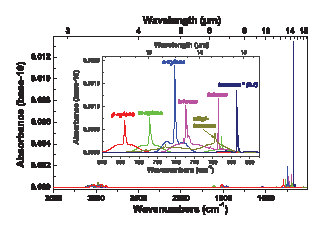
\includegraphics[width=5in]{chpt3/chpt3_btex}
\caption[Absorption spectra for BTEX molecules]{\textnormal{\textbf{Absorption spectra for BTEX molecules.}}  Compared with the fundamental vibrational absorption lines of most molecules, aromatic hydrocarbons have their strongest absorption lines at relatively long wavelengths.  Benzene, for example, has an especially strong absorption at $14.8~\tn{\um}$.  The absorption lines of BTEX compounds are spectrally distinct, providing an avenue for detection selectivity of these compounds.}
\label{chpt3:btex}
\end{figure}

The absence of RT CW QC laser sources with emission beyond 12~\um\ has not been for a lack of trying.  Pushing QC capabilities to longer wavelengths began as early as 1998, when C.\ Gmachl \emph{et al.} reported 13~\um\ emission from a convention single-phonon, three well active region QC structure \cite{Gmachl:EL:1998:13um}.  This laser operated up to a pulsed $T_{max}\approx175$~K.  In 1999, A.\ Tredicucci \emph{et al.} found the QC superlattice architecture well-suited for longer-wavelength emission, with the demonstration of lasing at 17~\um\ \cite{Tredicucci:APL:1999:17um}.  Superlattice structures later showed emission at 19~\um\ \cite{Tredicucci:APL:2000:19um} and then 21.5 and 24~\um\ \cite{Colombelli:APL:2001:24um}.  Each of these superlattice demonstrations exhibited a pulsed $T_{max}\approx140$~K.  Without question the best performance demonstrated by a long-wavelength QC laser was by M.\ Rochat \emph{et al.} at 16~\um\ \cite{Rochat:APL:2001} \cite{Kosterev:APB:2002:15um}.  For this ``bound-to-continuum'' structure, pulsed $T_{max}>333$~K.  Clearly, history has proven longer-wavelength light generation to be a substantial challenge.

%Today's ``upper limit'' on wavelength is a reduction in performance much more gradual than the lower limit imposed by the material band offsets.  Still, the technical challenges confronted in the quest for long-wavelength lasing are just as complex-perhaps more so.  The upper limit on wavelength, or at least the gradual decline in performance where the extension to longer wavelengths-lower photon energies-becomes extremely challenging.  has a different set of technical challenges from the short wavelength side

%Long--wavelength light generation ($\lambda~>$~12\um\ presents an especially daunting set of challenges to current QC technology.  Beyond 12~\um, laser performance falls off significantly, and no commercially--available QC sources exist.  Furthermore, CW RT performance beyond 12~\um has yet to be demonstrated.

%In fact, a large gap exists over the Restrahlan band of III--V.  There are important applications here, such as the strongest absorption lines for aromatic hydrocarbons (benzene is at 14.8~\um), many other organic and biologically relevant molecules, and other heavy molecules.  Best lasers at long wavelength.


\bigskip

In this chapter, I discuss a QC laser design strategy---namely the use of ``excited state'' optical transitions---intended to boost oscillator strength and thereby overcome many of the aggravating factors preventing high performance lasing at longer wavelengths.  While the excited state concept shows promise for such an effect, we discovered that these excited state QC structures are capable of simultaneous dual-wavelength lasing from two different optical transitions within the active region.  Furthermore, the secondary emission shows some extra--ordinary properties.  The interplay between charge carriers within the active region led to the secondary lasing transition being suppressed until a thermal turn-on; under certain circumstances, performance for the secondary emission actually \emph{improves} with temperature.  Ultimately, we found that the secondary emission is lasing only high in \emph{k}-space: the lasing originates from electrons in a highly non-equilibrium state.


\section{The Long-wavelength Challenge}

The technical hurdles confronted in the pursuit of long-wavelength lasing are perhaps even more daunting than those imposed by material band offsets at the short wavelength limit.  Two primary mechanisms---optical loss and decreased upper laser state lifetimes---%
%\begin{enumerate}
%\item optical absorption loss, and
%\item decreased upper laser state lifetimes %, and
%%\item decreased out--coupling efficiency,
%\end{enumerate}
individually compound in a situation that frustrates QC designs and performance at longer wavelengths.

\begin{figure}[tbp]
\centering
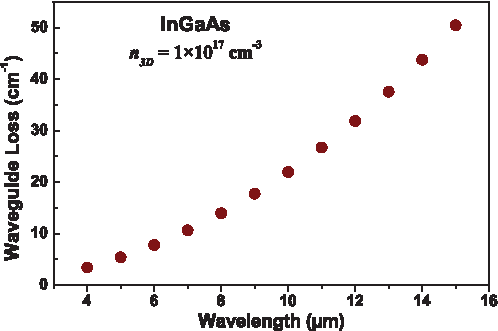
\includegraphics[width=4in]{chpt3/chpt3_wgloss}
\caption[Optical absorption of bulk InGaAs]{\textnormal{\textbf{Optical absorption of bulk InGaAs.}}  Calculated for In\sub{\textsf{0.53}}Ga\sub{\textsf{0.47}}As with a free electron density $n_{3D}=1.0\times10^{17}\tn{~cm}^{-3}$.  Waveguide loss increases super-linearly with wavelength.}
\label{chpt3:wgloss}
\end{figure}

Optical loss, or waveguide loss $\alpha_w$, is related to the complex refractive index $\textit{\~{n}}$ as
\begin{equation}
\alpha_w = 2 \frac{2 \pi \textrm{Im}[\textit{\~{n}}]}{\lambda_0} \text{.}
\end{equation}
In the long-wave infrared region, $\textit{\~{n}}$ is especially impacted by the presence of free carriers (\emph{i.e.}, electrons).  For bulk materials, $\textit{\~{n}}$ can be estimated using the Drude model.  Given a plasma frequency $\omega_p$ as
\begin{equation}
\omega_p=\sqrt{\frac{4\pi q^2 n_{3D}}{m^* \epsilon_{inf}}}
\end{equation}
which is dependent on the free electron density $n_{3D}$ and the electron effective mass $m^*$, the complex refractive index $\textit{\~{n}}$ is
\begin{equation}
\textit{\~{n}} = \sqrt{\epsilon_\infty\left(1-\frac{\omega_p^2}{\omega^2+\textrm{i} \frac{\omega}{\tau}}\right)}
\end{equation}
where $\tau$ is the mean collision time for free electrons, usually taken as 0.1~ps in III--V semiconductors.  A calculation for $\alpha_w$ in bulk In\sub{0.53}Ga\sub{0.47}As for a typical doping $n_{3D}=1\times10^{17}~$cm\sup{-3} shows the dramatic increase of waveguide loss with wavelength.  As shown in Fig.~\ref{chpt3:wgloss}, while at $\lambda=5$~\um\ the waveguide loss $\alpha_w\approx5$~cm\sup{-1} , at $\lambda=15$~\um, $\alpha_w\approx50$~cm\sup{-1}!

\begin{figure}[tb]%
\centering%
\subfloat[]{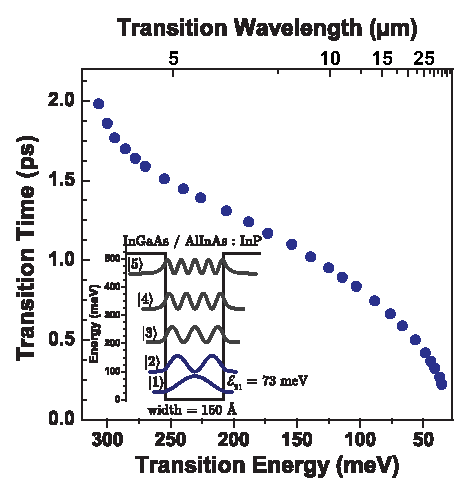
\includegraphics[width=2.9in]{chpt3/chpt3_lifetimea}%
\label{chpt3:lifetimea}}%
\hfil%
\subfloat[]{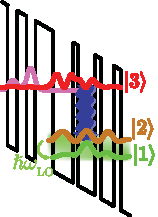
\includegraphics[width=1.8in]{chpt3/chpt3_lifetimeb}%
\label{chpt3:lifetimeb}}%
\caption[LO phonon lifetime vs.\ transition wavelength]{\textnormal{\textbf{LO phonon lifetime vs.\ transition wavelength.}}  \tn{\textbf{(a)}} For a single quantum well, the LO phonon scattering time is plotted for decreasing \trans{2}{1} transition energy $\EE_{21}$ (increasing transition wavelength). For $\hslash\omega_{LO}<34\tn{~meV}~(\approx36\tn{~\um})$, the small transition energy precludes scattering by LO phonons, the fastest scattering process in semiconductors. \tn{\textbf{(b)}} A schematic representation of a conventional single-phonon active region with optical transition \trans{3}{2} and phonon transition \trans{2}{1}.}
\label{chpt3:lifetime}
\end{figure}

The ability to attain population inversion also becomes more difficult at longer wavelengths.  A fundamental mechanism of most all QC lasers is the use of LO phonon scattering to rapidly depopulate the lower laser state.  For a generic three level QC active region, as in Fig.~\ref{chpt3:lifetimeb}, one seeks to position the lowest two energy states one LO phonon energy apart ($\EE_{21}\geq\hslash\omega_{LO}$); in InGaAs, $\hslash\omega_{LO}\approx34\textnormal{~meV}$ (equivalent to a wavelength of 36~\um).  As shown in Fig.~\ref{chpt3:lifetimea}, the LO phonon scattering time for $\EE_{21}=\hslash\omega_{LO}$ is about 0.2~ps.  For the optical transition (\trans{3}{2} in Fig.~\ref{chpt3:lifetimeb}), the lifetime due to phonon scattering decreases as the transition energy decreases.  %In this way, an intrinsic, built-in population inversion is designed into the QC device.
However, as $\EE_{32}$ approaches $\EE_{21}$, $\tau_{32}$ and $\tau_{2}$ become similar.  With population inversion (and therefore gain) proportional to $\left(1-\frac{\tau_2}{\tau_{32}}\right)$, maintaining the ability to achieve population is most definitely a concern at longer wavelengths.
%However, Fig. ? illustrates how this built-in inversion gets smaller as the wavelength of the optical transition nears the LO phonon energy.  For the single well example in Fig. ?, the ratio between the lifetime of a 5~\um transition to LO phonon lifetime is 9.0, whereas the ratio between the lifetime of a 15~\um transition to the LO phonon lifetime is 3.2.  With population inversion and therefore optical gain proportional to $(1-\frac{\tau_\ell}{\tau_{u\ell}})$, the effect of small photon energies on population inversion becomes evident.

%Say something about impedance mismatch.

The combination of small photon energies, high waveguide losses, and short upper-state lifetimes make long-wavelength QC lasers fundamentally inefficient devices.  From Chapter~2, wall-plug efficiency
\begin{equation}
\eta_{WPE} = \left(\frac{\EE_{ph}}{\EE_{ph}+\Delta_{inj}+\frac{q R_\textit{series}I}{N_p}}\right) \left(\frac{\alpha_m}{\alpha_w+\alpha_m}\right) \left(\frac{\tau_{eff}}{\tau_{eff}+\tau_2}\right) \left(\frac{J}{J-J_{th}}\right) \xi_{inj} \text{~.}
\end{equation}
The implications of long-wavelength lasing affect nearly every component term that contributes to the overall wall-plug efficiency.  The small photon energy $\EE_{ph}$ relative to the fixed values of $\Delta_\textit{inj}$ and $R_\textit{series}$ substantially reduce voltage efficiency.  And while high waveguide losses hurt the out-coupling efficiency, they also decrease current efficiency by increasing $J_{th}$.  Likewise, the short upper-state lifetimes increase $J_{th}$ and decrease current efficiency, in addition to decreasing transition efficiency term.


\section{Excited State Transitions}

A chief battle long-wavelength lasers must overcome is simply ``turning on''---\emph{i.e.}, reaching threshold---at a current density below $J_{max}$.  The challenges posed by long-wavelength lasing are in large part fundamental in nature; the effects of free carrier absorption and phonon lifetimes are built-in properties of the system.  However, many design parameters affected by the QC design itself are included in threshold current density:
\begin{equation}
J_{th}(T = 0) = \frac{\alpha_m + \alpha_w}{g\Gamma}
\end{equation}
where
\begin{equation}
g = \frac{4 \pi q}{\lambda_0 \epsilon_0 n_\textit{eff}} \frac{1}{\delta\!\EE_{u\ell}} \frac{\tau_u \left(1-\tau_\ell/\tau_{u\ell}\right)z_{u\ell}^2}{L_p} \text{~.}
%\delta_{u\ell} \frac{\epsilon_0 \lambda_0 n_\textit{eff}}{4 \pi q} \frac{L_p}{\Gamma} \frac{\alpha_m + \alpha_w}{\tau_u (1-\frac{\tau_\ell}{\tau_{u\ell}}) z_{u\ell}^2} \text{~.}
\end{equation}
If optical losses and phonon scattering times cannot be directly affected by clever design, another strategy might serve to compensate for these effects by boosting the values of other parameters.  For example, the optical dipole matrix element $z_{u\ell}$ contributes quadratically to the gain.  Thus, a modest increase in $z_{u\ell}$ can have a rather substantial overall impact on lowering $J_{th}$.


\begin{figure}[tb]%
\centering%
\subfloat[]{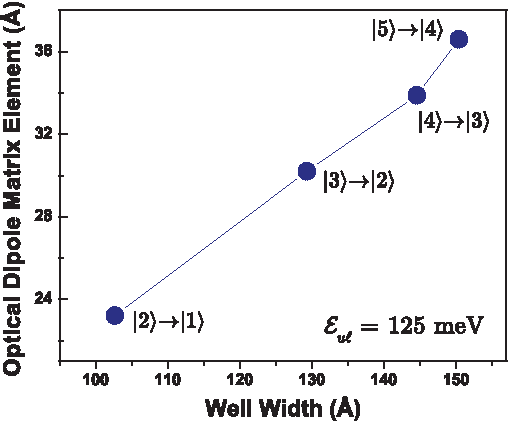
\includegraphics[width=2.9in]{chpt3/chpt3_dipolea}%
\label{chpt3:dipolea}}%
\hfil%
\subfloat[]{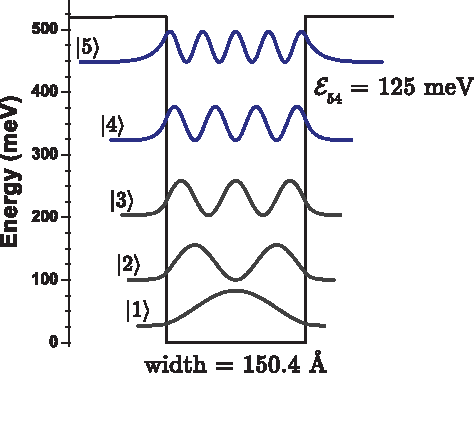
\includegraphics[width=2.3in]{chpt3/chpt3_dipoleb}%
\label{chpt3:dipoleb}}%
\caption[Optical dipole matrix elements for a single quantum well.]{\textnormal{\textbf{Optical dipole matrix elements for a single quantum well.}} \textnormal{\textbf{(a)}} The calculated optical dipole matrix element of the specified transition, where well width has been adjusted to give a transition energy $\EE_{u\ell}=125~\tn{meV}$. For this constant transition energy, the optical dipole matrix elements and quantum well widths increase for transitions between higher lying adjacent levels.  Here we simulate optical transitions in the InGaAs/AlInAs:InP system, which has a conduction band offset of \textnormal{520~meV}. \tn{\textbf{(b)}} An example configuration for the single quantum well calculation, where the \trans{5}{4} transition energy $\EE_{54}=125~\tn{meV}$ at a well width of \textnormal{150.4~\AA}.}%
\label{chpt3:dipole}%
\end{figure}

The optical dipole matrix element between two energy states $z_{u\ell}$ can be simplistically thought of as closely related to the amount of spatial overlap between those states: the more overlap, the larger is $z_{u\ell}$.  Using the example of a single quantum well, as in Fig.~\ref{chpt3:dipole}, it is interesting to observe the relation between various consecutive energy states and $z_{u\ell}$.  By keeping the transition energy constant---in this case $\EE_{u\ell}=125$~meV---we obtain a fair comparison of $z_{u\ell}$ for the ladder of adjacent energy states in the well. Clearly, $z_{u\ell}$ increases for higher-lying transitions.  In this example, $z_{21}=23.2$~\AA\ and $z_{32}=30.2$~\AA, suggesting a potential increase in gain by a factor of 1.7 (considering the quadratic contribution to optical gain) when using a \trans{3}{2} optical transition rather than a \trans{2}{1} transition.

Further examination of Fig.~\ref{chpt3:dipolea} suggests another benefit from using excited state transitions.  To keep the transition energy constant while climbing the ladder of transitions between adjacent states, the well itself must be widened.  Intuitively, wider wells mean that a relatively smaller portion of the upper laser state wavefunction is perturbed by inhomogeneity at well--barrier interfaces.  In most QC lasers, interface roughness-induced broadening is the dominant contributor to the gain spectrum width $\delta\!\EE_{u\ell}$ \cite{Tsujino:APL:2005:roughness}.  With $J_{th}$ being proportional to $\delta\!\EE_{u\ell}$, wider QC active region quantum wells can be expected to be a net benefit for laser performance.

By this logic, making use of ``excited state'' transitions---those made purely from quantum mechanical excited states---is a potential approach for increasing QC laser gain and decreasing threshold current densities.  Yet with the multitude of coupled quantum wells that make up a QC laser design, it may not be immediately clear what an excited state QC laser might look like.  In the case of the single quantum well in Fig.~\ref{chpt3:dipole}, identifying excited states is quite simple: the lowest energy state in the well is the ground state, and each state above the ground state is an excited state.  Thus, any transition not between \trans{2}{1} is an excited state transition.

\begin{figure}[tb]%
\centering%
\subfloat[]{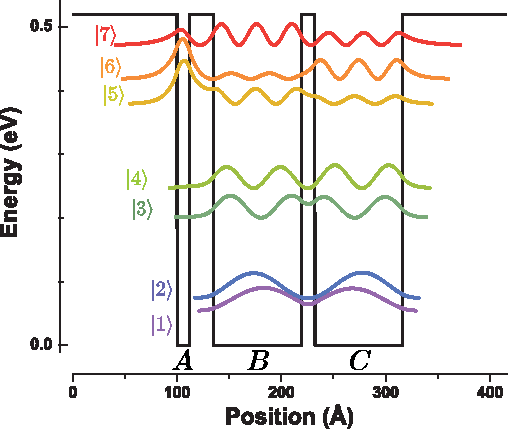
\includegraphics[width=2.6in]{chpt3/chpt3_es_pictoriala}%
\label{chpt3:es_pictoriala}}%
\hfil%
\subfloat[]{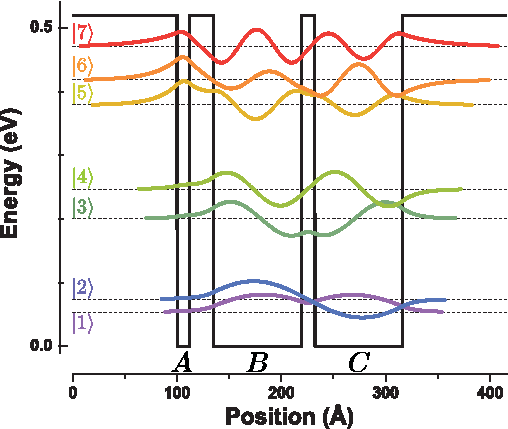
\includegraphics[width=2.6in]{chpt3/chpt3_es_pictorialb}%
\label{chpt3:es_pictorialb}}%
\caption[Energy state mixing in coupled quantum wells.]{\textnormal{\textbf{Energy state mixing in coupled quantum wells.}} A pictorial example of energy state mixing calculated for a three coupled quantum well In\sub{\textsf{0.53}}Ga\sub{\textsf{0.47}}As / Al\sub{\textsf{0.48}}In\sub{\textsf{0.52}}As system.  The quantity $\langle\psi(z)|\psi(z)\rangle$ is plotted in \tn{\textbf{(a)}} and $\psi(z)$ is plotted in \tn{\textbf{(b)}}.  States \ket{1} and \ket{2} are ground states, and \ket{3} and \ket{4} are first-excited states.  States \ket{5}, \ket{6}, and \ket{7} are largely second-excited states, with some ground state character in well \tn{\textit{A}}.}%
\label{chpt3:es_pictorial}%
\end{figure}

In the case of coupled quantum wells, what particularly matters for our characterization of excited state transitions is more the ``shape'' of the energy state, rather than an individual state's position relative to the other states in the system.  A pictorial example may be helpful.  In Fig.~\ref{chpt3:es_pictorial}, we have three coupled quantum wells; Fig.~\ref{chpt3:es_pictoriala} plots our usual $\langle\psi(z)|\psi(z)\rangle$ while Fig.~\ref{chpt3:es_pictorialb} plots $\psi(z)$.  As in our example of a single quantum well, each of the coupled quantum wells will contribute to the system an energy state that looks quantum mechanically like a ground state; that is, each coupled well contributes to the system one state with a shape having zero nodes within each coupled well.  Momentarily ignoring the narrow well \textit{A}, the states labeled \ket{1} and \ket{2} are the ``ground states'' for the coupled wells \textit{B} and \textit{C}.  Likewise, each coupled well will contribute one first-excited state; the states labeled \ket{3} and \ket{4} are ``first-excited states'' for the coupled wells \textit{B} and \textit{C}, since they each have one node within each coupled quantum well.  The characterization gets slightly more complicated when narrow wells are placed adjacent to wide wells (as in the case of a QC laser with the conventional narrow injector well adjacent to the first wide active region well).  This creates a situation where a ground state ``mixes'' with an excited state, such as the case for states \ket{5}, \ket{6}, and \ket{7}.  Each state in this group has zero nodes in well \textit{A}, but two nodes in wells \textit{B} and \textit{C}; over most of their probability densities, \ket{5}, \ket{6}, and \ket{7} are characteristically second-excited states, with some ground state shape in well \textit{A}.

Using this convention, most all QC lasers to date have used a first-excited state and ground state, respectively, for the upper and lower states of the laser transition.  For example, the now classic double-phonon design \footnote{For an example conventional double phonon band structure, see Fig.~\ref{chpt4:Razeghi}.} \cite{Beck:Science:2002} uses three wide active region wells, thus yielding three ground states \ket{3}, \ket{2}, and \ket{1}---with $\EE_{32}$ and $\EE_{21}$ roughly the energy of one LO phonon.  The upper laser state, conventionally labeled \ket{4}, is a first-excited state, making the laser transition \trans{4}{3} a first-excited state to ground state transition. There are, however, a few examples in the literature of QC lasers that have used optical transitions composed completely from excited states.  In an attempt to achieve a ``cascaded'' QC laser---that is, a QC active region with sequentially stacked optical transitions that would be a scheme for correlated photon generation \cite{Scully}---J.~Faist \textit{et al.} injected electrons into state \ket{3} of a single quantum well active region.  In this work, they observed lasing from \trans{3}{2}, an excited state transition similar to \trans{3}{2} in Fig.~\ref{chpt3:dipoleb}.  Notably, they were unable to achieve lasing from \trans{2}{1}.  More examples exist for THz QC lasers---lasers where $\hslash\omega_{ph}<\hslash\omega_{LO}$.  In a THz QC structure, G.~Scalari \textit{et al.} also observed stacked transitions; in this case different applied electric field values resulted in switching emission between \trans{3}{2} and \trans{4}{3}, yielding field-selectable output at either $\EE_{32}=5.75$~meV (1.39~THz) or $\EE_{43}=9.5$~meV (2.3~THz) \cite{Scalari:APL:2006}.


\section{Excited State QC Laser Design}

We have implemented an excited state QC laser design in a two-well active region configuration using In\sub{0.53}Ga\sub{0.47}As wells and Al\sub{0.48}In\sub{0.52}As barriers.  The conduction band energy diagram is shown in Fig.~\ref{chpt3:band_diagram}.  Rather than injecting electrons into state \ket{3} as in a conventional two-well (single-phonon) QC laser, our injector region is specifically designed on the downstream side to inject electrons into state \ket{5}.  Our optical transition is thus designed to be between states \ket{5} and \ket{4}; because \ket{5} is a second-excited state and \ket{4} is a first-excited state, the transition \trans{5}{4} is an excited state transition.  The design energy $\EE_{54}=128$~meV ($\lambda=9.68$~\um).  The injector region is also designed with relatively narrow barriers on the upstream side; these narrow barriers result in a large splitting of the injector states, intended to efficiently empty out the active region states \ket{4} through~\ket{1}.

\begin{figure}[tbp]
\centering
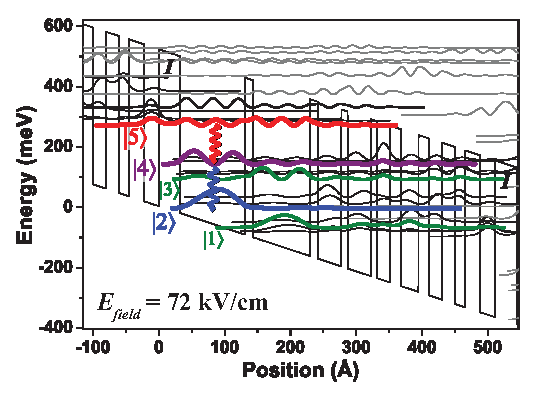
\includegraphics[width=5.25in]{chpt3/chpt3_band_diagram}
\caption[Excited state QC laser band diagram]{\textnormal{\textbf{Excited state QC laser band diagram.}}  Optical transitions are observed between states \trans{5}{4} and \trans{4}{2}.}
\label{chpt3:band_diagram}
\end{figure}

The laser was grown using gas-source molecular beam epitaxy on a low-doped ($n_{3D}<2\times10^{17}$~cm\sup{-3}) InP:S substrate.  The active core consisted of 40 active--injector region periods, and the design included 0.55~\um\ of \InGaAs (Si-doped $n_{3D}=5\times10^{16}$~cm\sup{-3}) for the cladding regions above and below the QC stack.  A 0.9~\um\ InP ($n_{3D}=5\times10^{16}$~cm\sup{-3}) buffer layer was grown before the bottom \InGaAs cladding. After the top \InGaAs cladding, additional cladding layers of 3.9~\um\ InP ($n_{3D}=5\times10^{16}$~cm\sup{-3}) and 1.1~\um\ InP ($n_{3D}=6.7\times10^{18}$~cm\sup{-3}) were grown, before capping the growth with 0.06~\um\ of \InGaAs ($n_{3D}=2\times10^{19}$~cm\sup{-3}).

The as-grown structure, plotted in the Fig.~\ref{chpt3:band_diagram} conduction band diagram is, in angstroms from the injection barrier, \textbf{32.3} / 97.7 / \textbf{12.9} / 86.0 / \textbf{12.9} / 35.2 / \textbf{9.7} / 35.2 / \textbf{9.7} / 19.5 / \textbf{16.1} / \underline{27.4} / \underline{\textbf{16.1}} / \underline{19.5} / \underline{\textbf{19.4}} / 15.6 / \textbf{22.6} / 23.5.  Here, \AlInAs layers are in bold type, \InGaAs layers are in plain type, and layers Si-doped $n_{3D}=2\times10^{16}$~cm\sup{-3} are underlined; the structure has an active core sheet density $n_s$~=~1.6~$\times$~10$^{11}$~cm$^{-2}$.

\begin{figure}[tbp]
\centering
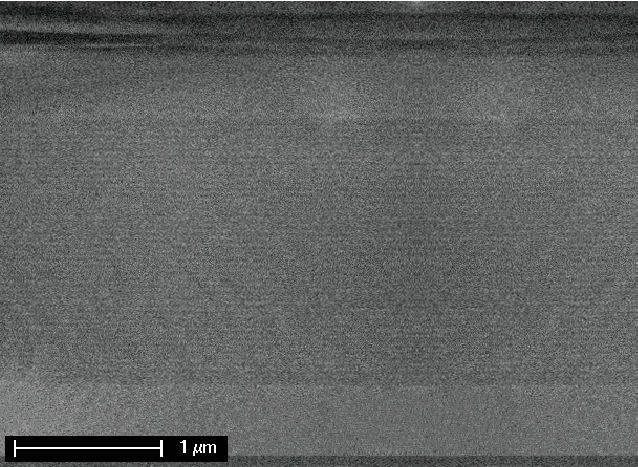
\includegraphics[width=4.25in]{chpt3/chpt3_sem}
\caption[SEM of excited state QC stack and waveguide]{\textnormal{\textbf{SEM of excited state QC stack and waveguide.}}  From bottom to top, color separations are seen representing the InP substrate, In\sub{\textsf{0.53}}Ga\sub{\textsf{0.47}}As bottom cladding, 40 period QC stack, In\sub{\textsf{0.53}}Ga\sub{\textsf{0.47}}As top cladding, and InP top cladding.}
\label{chpt3:sem}
\end{figure}

Following growth, we post-calibrated our structure by measuring active region and cladding layer thicknesses with high magnification scanning electron microscope (SEM) images, such as in Fig.~\ref{chpt3:sem}.  Here, we are able to see each individual QC period in the active core, along with the \InGaAs cladding layers, giving us an accurate measurement of the actual period thicknesses.  \InGaAs cladding thicknesses showed the \InGaAs growth rate was slow by a factor of 0.96 from the original calibration; the active core thickness showed the \AlInAs growth rate was slow by a factor of 0.80 from the original calibration.

To confirm accuracy of our post-calibrated structure, we analyzed the wafer with high resolution double crystal X-ray diffraction.  X-ray data show the primary InP reflection along with five satellite peaks that correspond to the QC core periodicity.  Analysis of the satellite peak positions shows a QC period length of 489.2~\AA\ with lattice mismatch of 0.04\%.  Our post-growth SEM-based characterization resulted in a period length of 511.3~\AA.  In comparing these two numbers, it is important to note that X-ray data was taken for a sample from the wafer edge, which generally has thinner layer thicknesses than the ``prime real estate'' of the wafer center.  The data set as a whole is consistent, since such a narrowing in layer thickness from center to edge is standard in MBE-grown material.

Lasers were processed as deep-etched ridge waveguides with stripe widths ranging from 9 to 15~\um\ by conventional photolithography and wet chemical etching, and were electrically insulated by 0.3~\um\ thick SiN\sub{x}. After evaporation of a Ti/Au (30~nm / 300~nm) top contact, the sample was thinned to $\sim\!200~\tn{\um}$ and a back Ge/Au (30~nm / 300~nm) contact was deposited. Laser bars were cleaved, mounted epitaxial-side up on Cu heat sinks with In solder, and wire bonded. Electroluminescence (semi-circular cleaved-mesa) devices were also fabricated.

%In the two-well active region laser presented here, we take the approach of using a second-excited state from one of the active region constituent quantum wells as the upper energy state of the first optical transition (state 5 in Fig. 1). The lower energy state of the first optical transition (state 4) is a first-excited state from one of the constituent quantum wells of the active region. This same state is also the upper state of the lower optical transition, making the two optical transitions "cascaded." The lowest energy state of the stacked optical transitions (state 2) is an active region constituent quantum well ground state. In the context of this specific QC laser description, we refer to a "ground state" as any state that originated from the true ground state of a constituent quantum well and accordingly for the excited states.


%We found our InAlAs growth rate to be slow by 20\%, and we have compensated for the difference in our design and simulations. The as-grown band structure is shown in Fig. 1.

%Simulation for the post-calibrated structure with a 65 kV/cm applied electric field results in an energy of 128.0 meV (  = 9.68 ?m) for the upper optical transition (levels 5?4) and an optical dipole matrix element of z54 = 31.0 �; we calculate an energy of 151.5 meV (  = 8.18 �m) for the lower optical transition (4?2) and an optical dipole matrix element of z42 = 14.4 �. The waveguide loss is estimated at 7.4 cm-1 for  = 9.68 �m and 5.1 cm-1 for   = 8.18 �m. The optical confinement factor for the active core is 60\% and 67\% for the two wavelengths, respectively. Considering longitudinal optical (LO) phonon scattering as the only scattering process, we calculate lifetimes  i of state i as  5 = 3.7 ps,  4 = 1.8 ps and  2 = 3.7 ps.

%The high k-space lasing reported here was discovered in an excited state QC laser16.  Excited state QC lasers are characterized in that the primary optical transition is engineered to be between energy states that both have the quantum mechanical attributes of constituent quantum well excited states (e.g., at least one wavefunction node per coupled quantum well)17.  In our two-well active region design, shown in the Fig. 1(a) conduction band energy diagram, the primary optical transition is between energy states labelled |5> and |4>; a conventional two-well QC laser design would use the states |3> and |2> for the optical transition.  A result of electrically injecting into highly excited active region states is that there inherently exist additional lower-lying energy levels with large oscillator strengths.  Below the states of the optical transition are three active region energy levels.  With electron injection high in the active region structure, these other levels are candidates for supporting additional optical transitions.

%Rate Equation Modeling
%Following Ref. 21, we modeled a system that considered carrier populations for levels |5>, |4>, |3>, |2>, and |1> as labeled in Fig. 1(a), along with high k-space populations for subbands |4> and |2>.  Photon densities from stimulated emission between transitions \trans{5}{4} and the high k-space \trans{4}{2} were also considered.  Given the waveguide structure, we calculate Drude-type optical free carrier losses $\tau$54 = 7.4 cm-1 and $\tau$42 = 5.2 cm-1 and confinement factors 54 = 0.60 and 42 = 0.67.  The full-width at half-maximum (FWHM) of the spontaneous emission is estimated from electroluminescence measurements at \EE54 = 24 meV and \EE42 = 15 meV.  Optical dipole matrix elements z54 = 23 Å and z42 = 13 Å are used.  Non-radiative LO-phonon scattering lifetimes are calculated to be 54 = 4.0 ps, 53 = 4.2 ps, 52 = 7.9 ps, 51 = 9.3 ps, 43 = 1.2 ps, 42 = 1.9 ps, 41 = 10.6 ps, 32 = 3.0 ps, 31 = 3.5 ps, and 21 = 7.2 ps.  We calculate the intrasubband scattering times at k = 3.6×108 m-1 for states |4> and |2> to be related by 4k/2k = 2.2 using a 1/k2 dependence (see main text); intrasubband lifetimes are assumed to be 4k = 0.99 ps and 2k = 0.45 ps.  Three fitting parameters are used, which each have independent effects on the model results.  First, optical loss for the \trans{5}{4} transition is scaled by a factor of 4.6; \trans{5}{4} threshold is largely unaffected by the remaining fitting parameters.  The scaling factor of 4.6 is reasonable given the known under-estimation of Drude absorption for free carrier loss.  Second, optical loss for the \trans{4}{2} transition is scaled by a factor of 0.1, which affects the modeled threshold for the \trans{4}{2} transition at temperatures higher than the threshold crossover.  Finally, the model assumes that 12\% of the injector ground state electrons directly populate the high k-space state |4>, with the balance being transferred via resonant tunneling into state |5>; this fitting parameter affects the modeled threshold for the \trans{4}{2} transition at temperatures lower than the threshold crossover.  Thus assuming, the \trans{4}{2} transition loss would conventionally have a similar scaling factor as the \trans{5}{4} transition loss, the overall improvement in loss from the high k-space transition is a factor of 46.


\section{Device Emission Characteristics}

\subsection{Electroluminescence and Identification of the Optical Transitions}

\begin{figure}[tbp]
\centering
\vspace*{-0.3in}
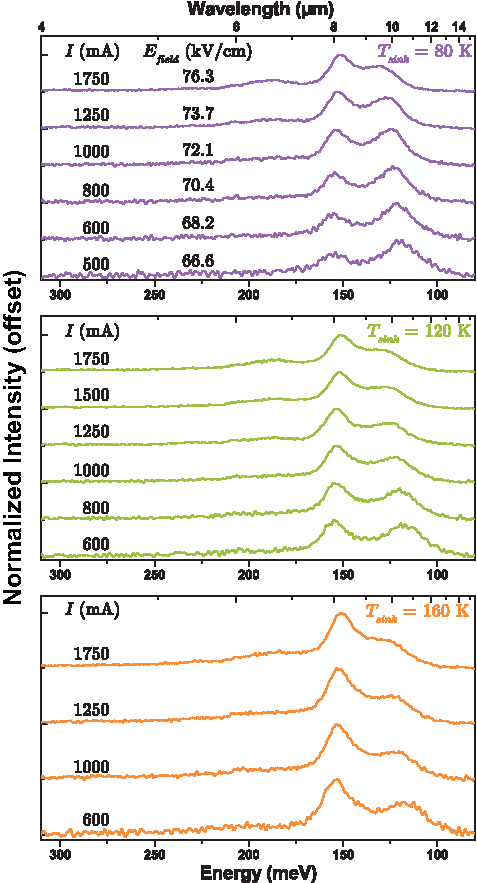
\includegraphics[width=4.25in]{chpt3/chpt3_el_spectra}
\caption[Excited state structure electroluminescence spectra]{\textnormal{\textbf{Excited state structure electroluminescence spectra.}}  Electroluminescence spectra from a $0.027~\tn{mm}^2$ semi-circular mesa.  Data were taken with current pulse width $t_{pulse}=100~\tn{ns}$ at an $80~\tn{kHz}$ repetition rate.}
\label{chpt3:el_spectra}
\end{figure}

Emission spectra for EL mesa structures were collected using an FTIR spectrometer in step scan mode.  Electroluminescence data are summarized in Fig.~\ref{chpt3:el_spectra} for heat sink temperatures $T_{sink}$ at 80, 120, and 160~K.  The data clearly show two distinct emission peaks, one near $\lambda\approx8$~\um\ and one near $\lambda\approx10$~\um.  At higher injection currents, higher photon energy emission is observed near $\lambda\approx6.5$~\um.  The two primary emission peaks have features largely independent of each other.  As both injection current and temperature increase, the $\sim\!8$~\um\ emission gets stronger in relation to the $\sim\!10$~\um\ emission.  Fitting Lorentzian line shapes to the individual peaks helps further quantify distinguishing characteristics.  As electric field changes, a clear Stark tuning is present for both emission peaks; however, the peaks tune in opposite directions.  As indicated in Fig.~\ref{chpt3:el_spectra} for $T_{sink}=80$~K and explicitly plotted in Fig.~\ref{chpt3:transID}, the $\sim\!10$~\um\ emission blue-shifts from 118 to 134~meV over an increasing applied field range of 15~kV/cm, while the $\sim\!8$~\um\ emission red-shifts from 156 to 152~meV over the same field range.  Such field-dependent behavior suggests that the $\sim\!10$~\um\ emission results from a transition that is rather diagonal in nature, while the $\sim\!8$~\um\ emission is from a transition that is more vertical.  The spectral widths of each peak additionally support diagonal and vertical origins for the $\sim\!10$ and $\sim\!8$~\um\ peaks. At $E_\textit{field}=72$~kV/cm, the $\sim\!10$~\um\ emission ($\hslash\omega_{ph}=125.6$~meV) has a FWHM $\delta\!\EE_{u\ell}=18.7$~meV $\left(\frac{\delta\!\EE_{u\ell}}{\hslash\omega_{ph}}=14.9\%\right)$ and the $\sim\!8$~\um\ emission ($\hslash\omega_{ph}=152.9$~meV) has $\delta\!\EE_{u\ell}=16.2$~meV $\left(\frac{\delta\!\EE_{u\ell}}{\hslash\omega_{ph}}=10.6\%\right)$. Because diagonal transitions are more heavily influenced by interface roughness, such transitions are expected to be spectrally broader \cite{Sirtori:OptLett:1998}.

\begin{figure}[tbp]
\centering
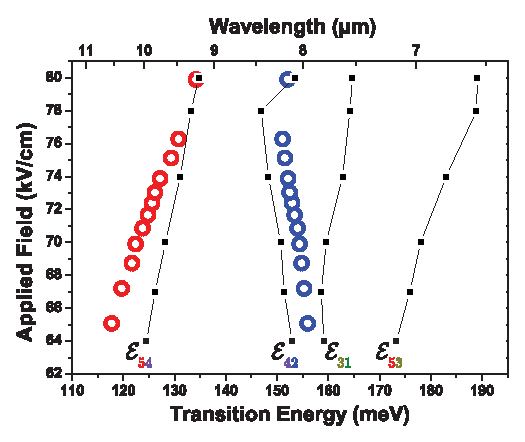
\includegraphics[width=4.25in]{chpt3/chpt3_transID}
\caption[Excited state transition identification]{\textnormal{\textbf{Excited state transition identification.}}  Measured and calculated values of the optical transition energies in EL as a function of the electric field.  Hollow circles represent the center points of multi-Lorentzian fits to the EL data as displayed in Fig.~\ref{chpt3:el_spectra} for $T_{sink}=80~\tn{K}$.  Solid squares show the calculated transition energies.}
\label{chpt3:transID}
\end{figure}

We identified the origin of the two transitions within the active region structure using the properties and behavior of the EL emission.  We calculated the energies and field-dependent behavior of all possible optical transitions within the structure, and in Fig.~\ref{chpt3:transID}, we show this data for the transitions \trans{5}{4}, \trans{4}{2}, \trans{3}{1}, and \trans{5}{3}.  As expected, our designed excited state \trans{5}{4} transition is the source of the 10~\um\ light.  Because both the field-dependent behavior and energies of the \trans{5}{3} and \trans{3}{1} transitions differ from the EL and laser spectra, we rule out these two transitions as the source of the $\sim\!8$~\um\ light. We thus identify the source of the $\sim\!8$~\um\ light to be the \trans{4}{2} transition; the unique field tuning behavior and the match in emission energy between observed and calculated data are in good agreement.


\begin{figure}[tbp]
\centering
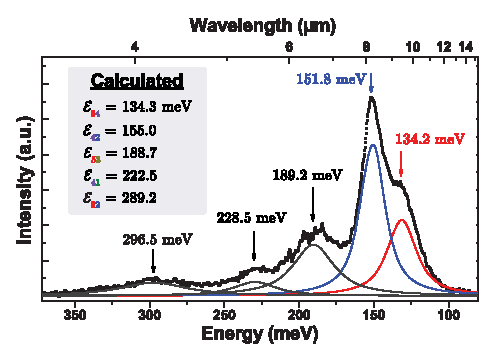
\includegraphics[width=4.25in]{chpt3/chpt3_fullEL}
\caption[EL at high pumping current]{\textnormal{\textbf{EL at high pumping current.}}  At $T_{sink}=80~\tn{K}$ and for $t_{pulse}=100~\tn{ns}$, the EL spectra at $2.5~\tn{A}$ for a $0.027~\tn{mm}^2$ device is fitted with five Lorentzian peaks.  The spectrum is shown without correction for detector responsivity.  Calculated transition energies are given for an electric field $E_{field}=80~\tn{kV/cm}$ and are in excellent agreement with the data.}
\label{chpt3:fullEL}
\end{figure}

As further verification of the accuracy of our calculations, we examined EL at high pumping current (2.5~A, 80~kV/cm).  Here, we observe five EL peaks, as shown with fitted Lorentzians in Fig.~\ref{chpt3:fullEL}.  We find excellent agreement between these peak positions and the calculated energies for the \trans{5}{4}, \trans{5}{3}, \trans{5}{2}, \trans{4}{2}, and \trans{4}{1} transitions.  We note that transitions from state \ket{3} are absent ($\EE_{32}=100.6$~meV and $\EE_{31}=163.4$~meV).  This is most likely due to a lack of electrons available to populate state \ket{3} as an optical transition upper state.


\subsection{Laser Emission}

We observe lasing from both transitions associated with the primary EL peaks \trans{5}{4} and \trans{4}{2}.  As with EL emission behavior, the two laser lines have distinctive and separate behavior.  Fig.~\ref{chpt3:lasing_spectra} shows laser emission at $T_{sink}=80$~K for a range of injection currents and pulse widths.  Noting that FTIR spectra are time-integrated, the emission changes from strongly favoring the \trans{5}{4} transition to strongly favoring the the \trans{4}{2} transition by changing the current pulse width $t_{pulse}$ from 10 to 100~ns.  That is, for $t_{pulse}=10$~ns, the \trans{4}{2} transition does not lase for $I\leq1.7$~A; for $t_{pulse}=100$~ns, the \trans{4}{2} threshold appears to be less than that of \trans{5}{4}.  Simultaneous lasing of both the \trans{5}{4} and \trans{4}{2} transition is seen for much of the parameter space.

\begin{figure}[tbp]
\centering
\vspace*{-0.3in}
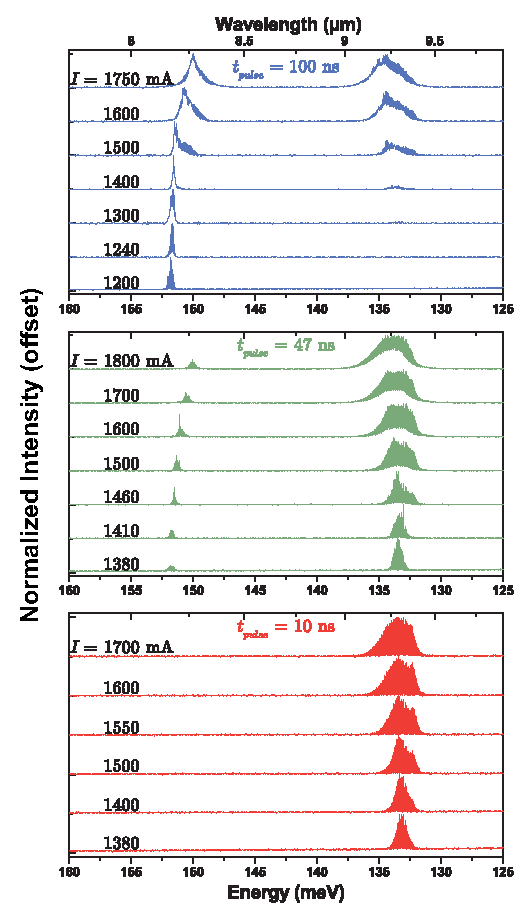
\includegraphics[width=4.25in]{chpt3/chpt3_lasing_spectra}
\caption[Excited state laser spectra]{\textnormal{\textbf{Excited state laser spectra.}}  Pulsed lasing spectra for a $2.5~\tn{mm}\times10~\tn{\um}$ laser ridge at a heat sink temperature $T_{sink}=80~\tn{K}$.  Current pulse widths $t_{pulse}$ were $10$, $47$, and $100~\tn{ns}$ at an $80~\tn{kHz}$ repetition rate.}
\label{chpt3:lasing_spectra}
\end{figure}

\subsection{Stacked Transitions}
Knowing our laser transitions are \trans{5}{4} and \trans{4}{2}, a re-examination of the band structure in Fig.~\ref{chpt3:band_diagram} illustrates how these transitions are energetically ``stacked.''  Indeed, with simultaneous lasing of both transitions, this appears to be the ``cascaded'' transition setup sought by C.\ Sirtori \emph{et al.} \cite{Sirtori:OptLett:1998} for producing correlated photons.  Besides the production of correlated photons, such stacked transitions could be useful for ultra-low noise spectroscopy applications, where the system noise of a secondary laser line is used to subtract out noise sources present in the laser line of primary interest.  Such an ability would result from the carrier populations of the two transitions being inherently linked.

While these applications certainly make the energy configuration represented in the Fig.~\ref{chpt3:band_diagram} band diagram highly interesting, the spectral data presented so far point to a problem with the interpretation.  In a relative sense, both EL and laser spectra show that when one transition becomes stronger, the other becomes weaker.  In the simple stacked transition picture, one would intuitively think that if one transition gets stronger, the other transition would also get simultaneously stronger; more carriers for one transition should yield carriers for the other.  In contrast to such output power behavior that is correlated, we observe just the opposite: anti-correlated behavior in output power.

\section{Anti-correlated Light Output Behavior}

Knowing that the two laser lines in the structure are substantially separated in wavelength, short-pass ($\lambda_{pass}<8.70~\tn{\um}$) and long-pass ($\lambda_{pass}>8.65~\tn{\um}$) filters were used to more thoroughly examine light vs.\ current (LI) characteristics of the laser devices.  In the LI data, the distinctive behavior of each transition becomes even more apparent, with light output and thresholds showing evident differences with remarkable temperature dependencies.

\begin{figure}[htbp]%
\centering%
\subfloat[]{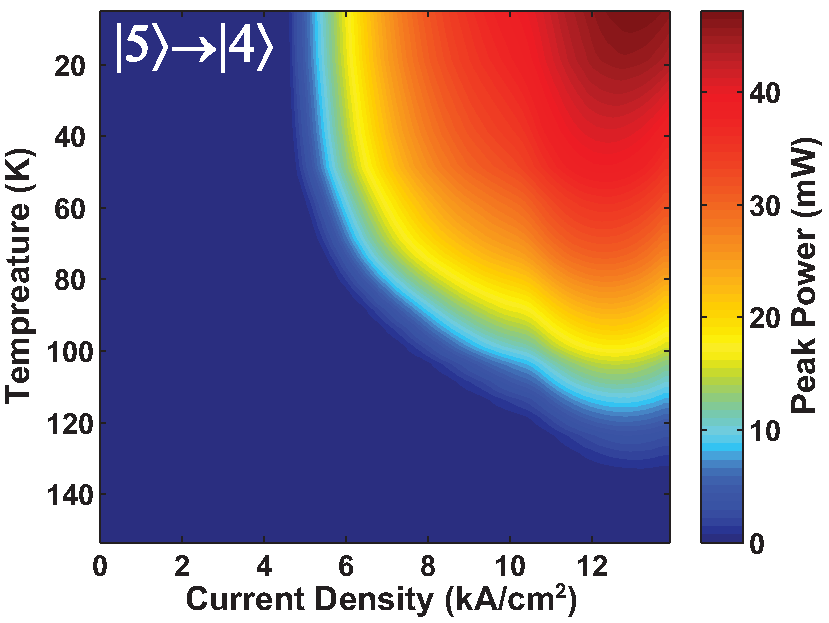
\includegraphics[width=4.1in]{chpt3/chpt3_li_54map}%
\label{chpt3:li_54map}}%
\\%
\subfloat[]{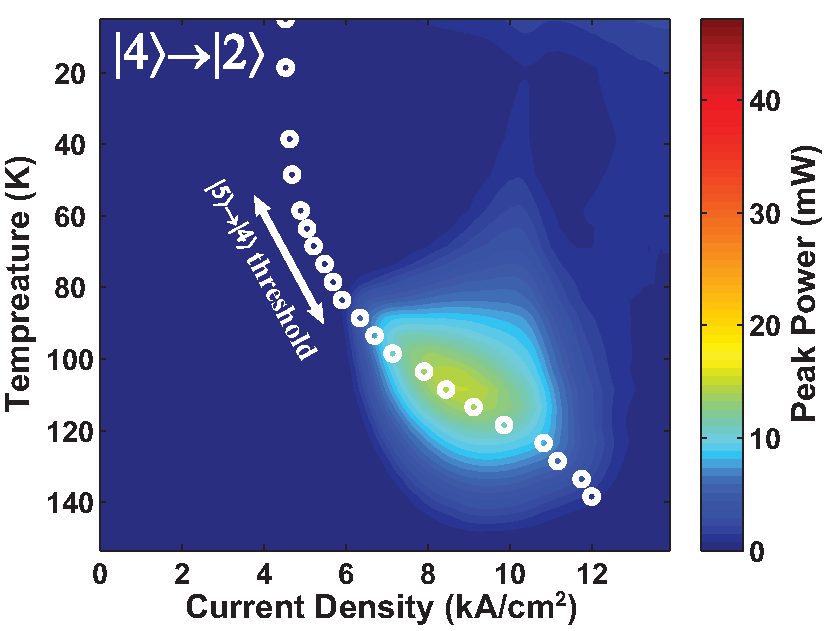
\includegraphics[width=4.1in]{chpt3/chpt3_li_42map}%
\label{chpt3:li_42map}}%
\caption[Light output characteristics of a representative laser device]{\textnormal{\textbf{Light output characteristics of a representative laser device.}} Light output versus current density and heat sink temperature of a $1.48~\textnormal{mm}\times12.1~\textnormal{\um}$ laser for the \tn{\textbf{(a)}} \trans{5}{4} and \tn{\textbf{(b)}} \trans{4}{2} transitions.  Data shown for the \trans{5}{4} transition are consistent with standard QC laser behavior.  In contrast, the \trans{4}{2} transition operates poorly at the lowest heat sink temperatures; the transition instead has a thermally induced peak performance near $115~\textnormal{K}$.  With the \trans{5}{4} transition threshold (white circles) overlaid on \tn{\textbf{(b)}}, it can be seen that the \trans{4}{2} roll-off is coincident with \trans{5}{4} turn-on.}%
\label{chpt3:li_maps}%
\end{figure}

Light from the \trans{5}{4} transition shows a behavior typical of a QC laser intersubband optical transition and is rather unremarkable.  As indicated in Figs.~\ref{chpt3:li_54map} and \ref{chpt3:li_crosssection}, the highest output power and lowest threshold currents are achieved at the lowest temperatures.  With increasing temperature, shorter non-radiative transition times, thermal population of the lower laser state, thermionic emission from the upper laser state, and decreased upper laser level injection efficiency make obtaining population inversion more difficult.  Consequently stronger pumping is required to achieve laser action, until a temperature is reached where the laser is unable to achieve threshold, in this case near $T_{sink}=125$~K \cite{Howard:JQE:2008}.

\begin{figure}[tbp]
\centering
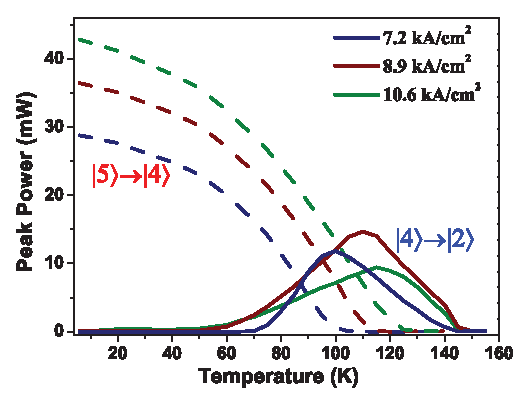
\includegraphics[width=4.25in]{chpt3/chpt3_li_crosssection}
\caption[Light--temperature cross-sections]{\textnormal{\textbf{Light--temperature cross-sections.}}  Spectrally resolved light output for three fixed pumping current densities with increasing temperature.  The \trans{5}{4} transition is shown with dashed lines and the \trans{4}{2} transition is shown with solid lines.  The \trans{4}{2} transition output is affected the the \trans{5}{4} transition outpu power.}
\label{chpt3:li_crosssection}
\end{figure}

\begin{figure}[tbp]
\centering
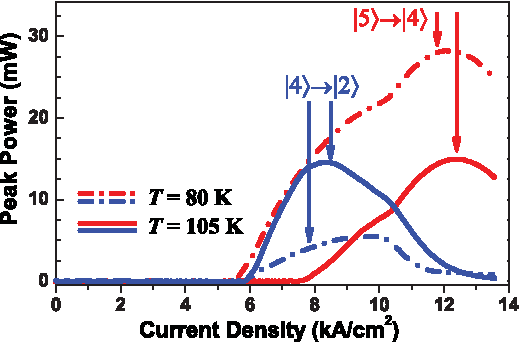
\includegraphics[width=4.25in]{chpt3/chpt3_li_anticorr}
\caption[Light--current cross-sections]{\textnormal{\textbf{Light--current cross-sections.}}  For each optical transition, light--current curves are shown at \textnormal{80} and $105~\textnormal{K}$.  A crossover in laser thresholds occurs at $85~\textnormal{K}$, where the \trans{4}{2} transition achieves a lower threshold than the \trans{5}{4} transition.  At $105~\textnormal{K}$, transition \trans{4}{2} has the lower threshold; here, the \trans{5}{4} transition threshold marks the beginning of the \trans{4}{2} power roll-off.}
\label{chpt3:li_anticorr}
\end{figure}

The lower \trans{4}{2} transition deviates from the familiar QC behavior significantly.  Most strikingly, the transition lases more effectively at elevated temperatures (near $T_{sink}=100$~K), while performance is substantially diminished at lower temperatures.  As shown in Figs.~\ref{chpt3:li_42map} and \ref{chpt3:li_crosssection} for a $1.48~\tn{mm}\times12.1~\tn{\um}$ device, lasing onset is induced near 60~K.  Peak output power with constant current density \emph{increases} with temperature up to 115~K, while threshold current simultaneously \emph{decreases}.  For temperatures above 115~K, a more typical thermal roll-over in power is observed.  The light--current curves in Fig.~\ref{chpt3:li_anticorr} reveal more:  a threshold ``crossover'' is observed at 85~K, above which point the \trans{4}{2} transition develops a lower threshold than the \trans{5}{4} transition.  At temperatures below this crossover, if the \trans{4}{2} transition is lasing, the \trans{5}{4} transition is also lasing.  After the crossover and for low pumping rates, a regime exists where only the lower \trans{4}{2} transition lases.  However, as soon as the upper \trans{5}{4} transition reaches threshold, an abrupt drop in \trans{4}{2} output power is observed.  This anti-correlation in output power between the two transitions persists even above threshold.  The Fig.~\ref{chpt3:crossover_data} plot of thresholds shows that after crossover, the \trans{4}{2} transition threshold takes on a more typical QC laser behavior, having a characteristic temperature $T_0\approx220$~K; before crossover, however, the transition has a \emph{negative} characteristic temperature $T_0\approx-66$~K\thinspace!  \enspace The sharp ``kink'' in the \trans{4}{2} transition threshold at the crossover point along with the anti-correlated output power behavior are indicative of a strong interaction between the carrier populations of the two laser transitions.

\begin{figure}[tbp]
\centering
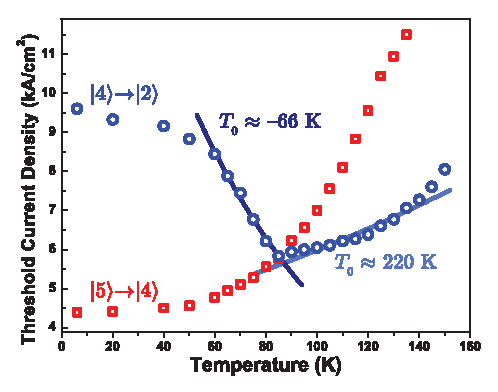
\includegraphics[width=4in]{chpt3/chpt3_crossover_data}
\caption[Threshold temperature-dependence of the transitions]{\textnormal{\textbf{Threshold temperature-dependence of the transitions.}}  Red symbols indicate observed threshold current densities for the \trans{5}{4} transition and blue symbols the \trans{4}{2} transition.  A crossover in thresholds is seen near $85~\textnormal{K}$.  Before this crossover, the \trans{4}{2} transition threshold decreases with increasing temperature, giving a negative characteristic temperature ($T_0\approx-66~\tn{K}$).  After the crossover, the \trans{4}{2} transition has a more conventional $T_0\approx220~\tn{K}$.}
\label{chpt3:crossover_data}
\end{figure}

For a thorough study of the structure, along with preliminary characterization of multiple ($\sim30$) laser devices, we performed full, detailed, temperature-dependent characterizations on six different lasers from different parts of the wafer.  Cavity lengths were 1.38, 1.48, 1.50, 1.63, 1.93, and 2.28~mm.  All data sets showed device characteristics similar to the data presented in Figs.~\ref{chpt3:li_maps}--\ref{chpt3:crossover_data}.  All devices showed anti-correlated behavior between two competing optical transitions lasing near $\lambda\approx9.5$~\um\ and 8.2~\um.  Also, a stronger \trans{5}{4} transition always led to a weaker \trans{4}{2} transition.




%Figure 2(a) shows time-integrated laser spectra collected using a Fourier Transform Infrared (FTIR) spectrometer. Spectra were taken using a current pulse width of 47 ns. The figure shows two distinct lasing peaks at   ~ 9.3 �m and   ~ 8.2 �m, in agreement with simulation for the transitions 5?4 and 4?2. With increasing electric field, the spectral distance between to the two lasing wavelengths narrows. Electroluminescence (EL) data exhibit similar characteristics. Deep, wet-etched, round mesas were patterned and processed, then cleaved into semi-circular structures to reduce optical feedback. The EL spectra-shown in Fig. 2(b)-exhibit two strong optical transitions that correspond to the two lasing wavelengths, and the peak centers show the same electric field tuning behavior as the laser devices. Fitting multiple Lorentzians for the 68 kV/cm spectrum gives a full-width at half-maximum (FWHM) of 18.7 meV for ~9.5 �m light and 16.2 meV for ~8.2 �m light. We note that state 5 extends over several interfaces, which can account for the broader 5?4 transition. Simulated electric field behavior of our structure is consistent with the observed data. The open circles in Fig. 3 represent multi-peak Lorentzian fits from EL data as in Fig. 2(b). Squares depict simulated energies of four possible transitions. As expected, the ~9.5 �m light results from transition 5?4.

%We observe two distinct optical transitions in the spontaneous emission spectrum: one at  ≈ 9.5 µm (near the original \trans{5}{4} design wavelength of 9.7 µm) and one at 8.2 µm, as shown in Fig. 1(b) for devices at 80 K.  With ridge laser structures at 80 K, we find that these transitions lase simultaneously; similar threshold currents are observed at this temperature.  We have previously identified14 the 9.5 µm emission as originating from transition \trans{5}{4} and the 8.2 µm emission originating from transition \trans{4}{2}, based on the resonant wavelengths of the emission spectrum and the unique field-dependent behaviour of the optical emission.

%Inspection of the Fig. 1 band structure confirms that the optical transition 5?4 is diagonal in nature while the 4?2 transition is vertical.  Simulated electric field behavior of our structure is consistent with the observed data.  The open circles in Fig. 3 represent multi-peak Lorentzian fits from EL data as in Fig. 2(b).  Squares depict simulated energies of four possible transitions.  As expected, the ~9.5 �m light results from transition 5?4.  Because both the field behavior and energies of the 5?3 and 3?1 transitions differ from the EL and laser spectra, we rule out these two transitions as the source of the ~8.2  m light.  We thus determine that the transition 4?2 is the source of the ~8.2 �m light.  At a current of 2.5 A (80 kV/cm), we observe five EL peaks, shown in Fig. 4.  A multiple-Lorentzian fit locates these peaks at 135 meV, 153 meV, 191 meV, 230 meV, and 299 meV.  Table I shows the simulated values for energy transitions at 80 kV/cm and the corresponding transition assignments.  We find excellent agreement between observed and simulated data.



\section{Lasing High in \textit{k}-Space}

\begin{figure}[tbp]
\centering
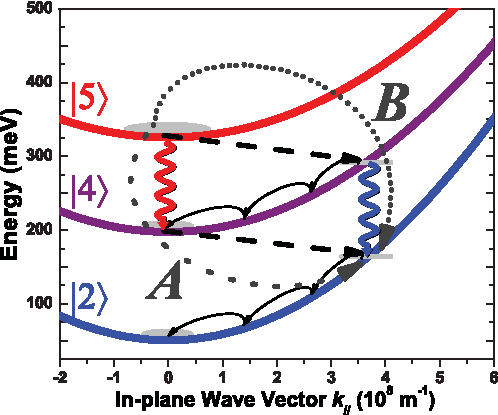
\includegraphics[width=5.25in]{chpt3/chpt3_electron_path}
\caption[The \emph{k}-space electron paths]{\textnormal{\textbf{The \emph{k}-space electron paths.}}  The in-plane \emph{k}-space dispersion $k_{/\!/}$ of the subbands \ket{5}, \ket{4}, and \ket{2} is shown.  Electrons being injected into state \ket{5} can follow either path \tn{\emph{A}} (the \trans{5}{4} optical transition) or path \tn{\emph{B}} (the \trans{4}{2} optical transition preceded by LO phonon scattering).  Path \tn{\emph{A}} is typical for a QC laser transition, and path \tn{\emph{B}} represents the high \emph{k}-space transition.  Optical transitions are indicated by wavy arrows, intersubband phonon transitions are shown with dashed-line arrows, intrasubband scattering is shown with curved arrows, and paths \tn{\emph{A}} and \tn{\emph{B}} are shown with dotted arrows.  Local \emph{k}-space minima (\emph{i.e.}, ``electron pools'') are shown as gray areas.}
\label{chpt3:electron_path}
\end{figure}

The simple stacked transition representation suggested by Fig.~\ref{chpt3:band_diagram} cannot account for the observed anti-correlated behavior in output power.  As earlier mentioned, such a stacked transition scheme would more directly lead to correlated---rather than anti-correlated---behavior in output power.  Our typical representation of the energy band configuration, such as in Fig.~\ref{chpt3:band_diagram}, hides many characteristics of the system.  Specifically, the system only has energy state quantization in one dimension, the direction of epitaxial growth.  In the other two (``in-plane'') dimensions, electrons are free to take on a much broader range of momentum (and therefore energy) values.  This in-plane freedom of motion creates an energy dispersion of the individual subbands of roughly parabolic form. Generally, any consideration of such dispersion is neglected in our energy band diagrams, since only the energy values at the energy band minima---the $\Gamma$ point ($k=0$)---are indicated by the plot.  In most cases, the simple picture is good enough, since most opto-electronic devices operate using electrons in a quasi-equilibrium state, or in a state where electrons are able to ``pool'' for a long time relative to other relevant system times.

%We used standard laser rate equations with stimulated emission terms to model a system with two optical transitions, including temperature-dependent parameters where appropriate.  The models show that population inversion for the \trans{4}{2} transition is not feasible with a practical parameter set for a purely stacked transition scheme where both transitions lase from the  point (k = 0).

The data presented in the previous sections require that we envision a mode of operation whereby a second optical transition is in competition with a first transition for charge carriers.  In a QC structure such as ours, we arrive at the model schematically depicted in Fig.~\ref{chpt3:electron_path}: the secondary laser transition is a vertical transition between subbands, positioned high in \emph{k}-space.  Given the three identified energy subbands \ket{5}, \ket{4}, and \ket{2}, several different electron transport paths are possible; two are labeled \emph{A} and \emph{B}.  Path \emph{A} is characteristic for a QC laser optical transition, where electrons undergo a radiative transition followed by LO phonon scattering.  When the \trans{5}{4} transition is lasing, large cavity photon densities at the \trans{5}{4} transition energy and strong stimulated emission ensure that this is the dominant electron path.  However, at elevated temperatures, path \emph{B} becomes available with increased LO phonon scattering out of state \ket{5}, populating state \ket{4} high in \emph{k}-space.  In the situation where path \emph{A} is ``off'' because threshold has not yet been reached for the \trans{5}{4} transition, carriers are provided so that lasing can occur at high \emph{k}-space for the \trans{4}{2} transition.  If at any time path \emph{A} turns on, path \emph{B} and therefore \trans{4}{2} population inversion is suppressed because
\renewcommand{\theenumi}{\roman{enumi}}
\renewcommand{\labelenumi}{(\theenumi)}
\begin{enumerate}
  \setstretch{1.0}
  \setlength{\itemsep}{0pt}
%  \setlength{\parskip}{0pt}
%  \setlength{\parsep}{0pt}
\item fewer electrons are available to populate the upper state of the high \emph{k}-space \trans{4}{2} optical transition and
\item electrons are injected into the lower state of the high \emph{k}-space \trans{4}{2} transition.
\end{enumerate}
Moreover, if transport through path \emph{A} is slowed due to a weakening \trans{5}{4} laser transition, path \emph{B} will concurrently see an enhancement of available electrons able to contribute to \trans{4}{2} lasing.  This effect accounts for the dramatic decrease in \trans{4}{2} threshold from 55 to 85~K.  The observed anti-correlated behavior of the two transitions is thus sustained.
It is worth noting that this anti-correlated transport picture implies that the \trans{4}{2} transition has only ``local'' population inversion; that is, population inversion does not exist globally over the entire subbands \ket{4} and \ket{2}.  This is not the first time local population inversion has been reported.  J.~Faist \emph{et al.} reported such local inversion in 1996 \cite{Faist:PRL:1996:local}.  However, their report detailed local inversion at $k=0$.  In contrast, our structure does not attain inversion at $k=0$ at all, and instead only reaches a local population inversion at high \emph{k}-space values.

The energy subband dispersion $\EE_{n}(k_{/\!/})$ plotted in Fig.~\ref{chpt3:electron_path} for subbands $n$ incorporates the energy dependence of the effective mass.  We define $\EE_{n}(k_{/\!/})$ relative to the conduction band edge as $\EE_{n}(0)$ (the subband energy at $k=0$) plus a dispersion term $\delta\!\EE_{n}(k_{/\!/})$,
\begin{equation}
\EE_{n}(k_{/\!/}) = \EE_{n}(0) + \delta\!\EE_{n}(k_{/\!/})
\end{equation}
and
\begin{equation}
\delta\!\EE_{n}(k_{/\!/}) = \frac{\hslash^2 k_{/\!/}^2}{2 m^*\!\bigl(\EE_{n}(k_{/\!/})\bigr)} = \frac{\hslash^2 k_{/\!/}^2}{2 \left(1+\frac{\EE_{n}(0) + \delta\!\EE_{n}(k_{/\!/})}{\EE_G^\Gamma}\right) m_e^*}
\end{equation}
using here the empirical approach of Nelson \emph{et al.} \cite{Nelson:PRB:1987} where $m^*\left(\EE\right) = \left(1+\frac{\EE}{\EE_G^\Gamma}\right) m_e^*$.  In the calculation for Fig.~\ref{chpt3:electron_path}, we use a $\Gamma$-point bandgap $\EE_G^\Gamma=0.784$~eV (which corresponds to a non-parabolicity parameter $\gamma=\frac{\hslash^2}{2 m_e^* \EE_G^\Gamma}=1.13\times10^{-14}~cm^2$ \cite{Sirtori:PRB:1994}) and assume the band-edge effective mass to be that of the \InGaAs well ($m_e^*=0.043 m_e$).

Making the assumption that $\hslash\omega_{LO}=34$~meV, electrons scattering out of state \ket{5} (at $k=0$) into state \ket{4} via LO phonons acquire a \emph{k}-space value $k_{/\!/}=3.6\times10^8$~m\sup{-1}.  We therefore infer that the observed high \emph{k}-space lasing occurs near $k_{/\!/}=3.6\times10^8$~m\sup{-1}, which is further supported by evidence described in the next section.  It is worthwhile to note that at $k_{/\!/}=3.6\times10^8$~m\sup{-1}, $\delta\!\EE_{4}(k_{/\!/})\approx90$~meV, giving about three LO phonon intrasubband scattering events before the electron reaches the quasi-equilibrium point at $k=0$.  Likewise, $\delta\!\EE_{2}(3.6\times10^8~\tn{m}^{-1})\approx113$~meV, again giving roughly three LO phonon events before the a high \emph{k}-space electron reaches the quasi-equilibrium point in subband \ket{2}.

This energy-dependence of the effective mass results in ``non-parabolicity'' of the energy subbands, a diversion of the energy subband from the truly parabolic shape proportional to $k_{/\!/}^2$ when effective mass has no energy dependence.  In our particular device, this non-parabolicity effect results in some highly interesting consequences.


\section{Effects of Non-parabolicity}
\label{chpt3:section_nonparabolicity}

\begin{figure}[tbp]
\centering
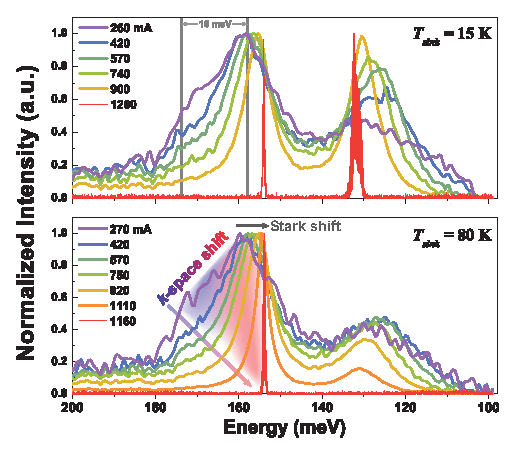
\includegraphics[width=4.75in]{chpt3/chpt3_redshift}
\caption[Spectral signature of \emph{k}-space emission]{\textnormal{\textbf{Spectral signature of \emph{k}-space emission.}}  Spectral behavior of a $1.93~\textnormal{mm}\times9.4~\textnormal{\um}$ laser at $15$ and $80~\textnormal{K}$, with the \trans{4}{2} transition emission centered around $160~\textnormal{meV}$.  Resulting from subband non-parabolicity, high \emph{k}-space emission has less photon energy than emission from $k=0$.  For the \trans{4}{2} transition, the broad emission with pronounced asymmetry at low injection currents is indicative of optical emission originating from a distribution of $k$ values.  As the injection current increases, the transition preferentially emits photons at the low-energy edge of the distribution---that is, from high in \emph{k}-space.}
\label{chpt3:redshift}
\end{figure}

Of particular interest for such a high \emph{k}-space transition is the effect of energy subband non-parabolicity \cite{Serapiglia:APL:2000:kspace}.  At the Brillouin zone center $k=0$, energy subbands have a substantially parabolic form.  However, non-parabolicity implies that, with both increasing $k$ and increasing subband energy above the band edge, the subbands flatten \cite{Sirtori:PRB:1994}.  This non-parabolicity has spectral consequences: for a transition between two subbands, the transition energy decreases as the transition occurs at higher $k$ values.  For the \trans{4}{2} transition in our structure, we calculate that photons generated at $k_{/\!/}=3.6\times10^8$~m\sup{-1} will have 16.1~meV less energy than photons generated at $k=0$.  Sub-threshold spectral data, as shown in Fig.~\ref{chpt3:redshift} for a $1.93~\tn{mm}\times9.4~\tn{\um}$ laser, reveal such a \emph{k}-space spectral signature.  For the \trans{4}{2} emission around 160~meV, we observe two effects that contribute to a spectral red-shift.  Over a range of injection currents that spans deeply sub-threshold to just above threshold, Stark tuning shifts the peak emission by $\sim\!5.5$~meV.  More interestingly, at low injection currents, the \trans{4}{2} emission exhibits pronounced asymmetry.  At the lowest injection currents, the spectral width is quite broad: about 16~meV.  As injection current is increased, the higher energy side of the emission collapses; the transition strongly favors emission on the side of low energy.  Also, as injection current is increased, the emission asymmetry gives way to a more typical Lorentzian-shaped emission.  Thus, for a laser device where cavity effects strongly influence emission behavior, these spectral features are consistent with laser emission originating high in \emph{k}-space.

Non-parabolic energy subbands lead to two interesting and favorable consequences for an electrically-pumped high \emph{k}-space laser transition.  Firstly, threshold currents are reduced due to a decrease in the primary source of optical absorption loss---that is, intersubband absorption at the lasing energy from the electron pool at $k=0$.  With a high \emph{k}-space transition between non-parabolic energy subbands, the optical emission process is decoupled from the normally concurrent reverse process of optical absorption.  Secondly, the presence of non-parabolicity helps achieve a more favorable lifetime profile for the \trans{4}{2} transition.  Because of non-parabolicity, the energy conversion of an LO phonon requires the exchange of a larger $k$ values for higher energy subbands, which in turn reduces the scattering rate \cite{Alcalde:PRB:1997} \cite{Ridley} \cite{Sinning:APL:2005} as $1/k^2$ \cite{Harrison} \cite{Bockelmann:PRB:1990}.  The influences of these effects are reflected in the results of our rate equation model.  As detailed in the next section, to reconcile calculated temperature-dependent thresholds with observed data, the optical absorption loss associated with the \trans{4}{2} laser energy was decreased by about a factor of 10.

Prior work on the theory of QC laser gain spectra \cite{Gorfinkel:JQE:1996} hinted at the feasibility of such an electrically-pumped high \emph{k}-space laser transition.  Here, Gorfinkel \emph{et al.} predicted the existence of local high \emph{k}-space population inversion resulting purely from the presence of energy subband non-parabolicity.  Because higher-energy subbands are ``flatter,'' the assumption of thermally-distributed \emph{k}-space energy dispersion implies that an inverted population profile can exist at high \emph{k}-space values even if the higher energy subband contains less total carriers than the lower subband.  In the work presented in this chapter, rather than relying on a thermal distribution of electrons around $k=0$ to populate a high \emph{k}-space energy band, our excited state QC design directly injects non--quasi-equilibrium high \emph{k}-space electrons.


\section{Rate Equation Modeling}

\subsection{A System of Two Coupled Optical Transitions}

To further confirm the plausibility of our \emph{k}-space interpretation, we modeled our laser with a common rate equation methodology.  Our rate equation model includes electron populations for six energy ``levels'': four for each of the active region energy levels \ket{5}, \ket{4}, \ket{3}, and \ket{2} in Fig.~\ref{chpt3:band_diagram}, and two high \emph{k}-space regions for subbands \ket{4} and \ket{2}.  The model also includes stimulated emission terms and photon fluxes for the transitions \trans{5}{4} and \trans{4}{2}.  The temperature dependence of energy state lifetimes \cite{Gmachl:review}, injection efficiency, thermal backfilling of energy states \cite{Gmachl:review}, and thermionic emission \cite{Sze} were all included.  Using the symbolic math toolbox in Matlab, we solved the system of rate equations under steady state conditions $\left(\frac{d (~)}{d\!t}=0\right)$.
\begin{equation}
\begin{split}
\setstretch{2}
\frac{d n_5}{d\!t} &=\eta_\textit{inj} \frac{J}{q}-n_5\left(\frac{1}{\tau_{54}}+\frac{1}{\tau_{53}}+\frac{1}{\tau_{52}}+\frac{1}{\tau_{51}}\right) -\frac{n_5}{\tau_{therm}} - S_{54} g_{54} \left(n_5-n_4\right)\\
\frac{d n_{4k}}{d\!t} &= \left(1-\eta_\textit{inj}\right) \frac{J}{q} + \frac{n_5}{\tau_5}-\frac{n_{4k}}{\tau_{4k}}-S_{42} g_{42}\left(n_{4k}-n_{2k}\right)\\
\frac{d n_4}{d\!t} &= \frac{n_{4k}}{\tau_{4k}} - n_4 \left(\frac{1}{\tau_{43}}+\frac{1}{\tau_{42}}+\frac{1}{\tau_{41}}\right) + S_{54} g_{54} \left(n_5-n_4\right)\\
\frac{d n_3}{d\!t} &= \frac{n_5}{\tau_{53}}+\frac{n_4}{\tau_{43}} -n_3 \left(\frac{1}{\tau_{32}}+\frac{1}{\tau_{31}}\right)\\
\frac{d n_{2k}}{d\!t} &= \frac{n_5}{\tau_{52}}+\frac{n_4}{\tau_{42}}+\frac{n_3}{\tau_{32}}-\frac{n_{2k}}{\tau_{2k}} +S_{42} g_{42} \left(n_{4k}-n_{2k}\right)\\
\frac{d n_2}{d\!t}&= \frac{n_{2k}}{\tau_{2k}}-\frac{n_2}{\tau_{21}}+\frac{n_{inj} e^{-\frac{\Delta_{inj}+\EE_{21}}{k T}}}{\tau_{21}}\\
\frac{d S_{54}}{d\!t} &= \left(N_p g_{54}\left(n_5-n_4\right)-\frac{1}{\tau_{ph1}}\right) S_{54}\\
\frac{d S_{42}}{d\!t} &= \left(N_p g_{42}\left(n_{4k}-n_{2k}\right)-\frac{1}{\tau_{ph2}}\right) S_{42}
\end{split}
\end{equation}
The temperature-dependence of all energy state lifetimes $\tau_{u\ell}$ was included with the standard relation derived from by the Bose--Einstein occupation of LO phonons.
\begin{equation}
\frac{1}{\tau_{u\ell}(T)} = \frac{1}{\tau_{u\ell}(0)} \left(1+\frac{2}{e^{\frac{\hslash\omega_{LO}}{k_B T}}-1}\right)
\end{equation}
The injection efficiency $\eta_\textit{inj}$ into the upper laser state \ket{5} (and into the \emph{k}-space state \ket{4}) \cite{Faist:SMM:book} was treated in a similar manner.
\begin{equation}
\eta_\textit{inj}(T) = \eta_\textit{inj}(0) \left[1-\left(1+\frac{2}{e^{\frac{\hslash\omega_{LO}}{k_B T}}-1}\right)\right]
\end{equation}
Thermionic emission out of the upper laser state \ket{5} was included using the method of S. Sze \cite{Sze}.
\begin{equation}
\tau_{therm}(T) = w \sqrt{\frac{2\pi m^*}{k_B T}} e^{\frac{\EE_{3c}}{k_B T}}
\end{equation}
The gain coefficient $g_{u\ell}$ for the transition \trans{u}{\ell} is given by
\begin{equation}
g_{u\ell} = \frac{c \Gamma_{u\ell}}{N_p n_\textit{eff}} \frac{2 q^2 \EE_{u\ell} z_{u\ell}^2}{h c \epsilon_0 n_\textit{eff} \; \delta\!\EE_{u\ell} L_p}
\end{equation}
and the photon lifetime with the cavity for the transition \trans{u}{\ell} is
\begin{equation}
\tau_{ph,u\ell} = \frac{n_\textit{eff}}{c \left(-\frac{1}{L} \ln(R) + \alpha_{w,u\ell} \right)} \text{.}
\end{equation}
The parameters used for the calculation are given in Tables~\ref{chpt3:tab1} and \ref{chpt3:tab2}.

\begin{table}[tbp]
\captionsetup{width=4in}
\centering
\setstretch{1.2}
\caption[Input parameters for the \emph{k}-space model]{Parameters used in the \emph{k}-space laser rate equation model.}
\vspace{-0.1in}
\begin{tabular*}{4in}{@{\extracolsep{\fill}} c c p{0.5in} c c }
\toprule
$R$ & 0.27 & & $L_p$ & 511~\AA\\
width & 12~\um & & $N_p$ & 40\\
$L$ & 1.5~mm & & $\Delta_\textit{inj}$ & 27.3~meV\\
$\hslash\omega_{LO}$ & 34~meV & & $n_\textit{inj}$ & $1.6\times10^{11}$~cm\sup{-3}\\
$\EE_{21}$ & 67.4~meV & & $\EE_{3c}$ & 60~meV\\
$w$ & 197~\AA & & $m^*$ & $0.043 m_e$\\
\hline
$\Gamma_{54}$ & 0.60 & & $\Gamma_{42}$ & 0.67\\
$\alpha_{w54}$ & 7.4~cm\sup{-1} & & $\alpha_{w42}$ & 5.2~cm\sup{-1}\\
$\EE_{54}$ & 128~meV & & $\EE_{42}$ & 151~meV\\
$z_{54}$ & 23~\AA & & $z_{42}$ & 13~\AA\\
$\delta\!\EE_{54}$ & 24~meV & & $\delta\!\EE_{42}$ & 15~meV\\
\hline
\end{tabular*}
\label{chpt3:tab1}
\end{table}

\vspace{0.5in}

\begin{table}[tbp]
\captionsetup{width=2.75in}
\centering
\setstretch{1.2}
\caption[LO phonon lifetimes used in the \emph{k}-space model.]{Calculated LO phonon lifetimes at $T=0~\tn{K}$ used in the \emph{k}-space laser rate equation model.}
\vspace{-0.1in}
\begin{tabular*}{2.75in}{@{\extracolsep{\fill}} c c | c c c c}
\toprule
\multicolumn{2}{c}{\multirow{2}{*}{\setstretch{0.9} \centering\parbox{0.2in}{$\tau_{u\ell}$\\(ps)}}} & \multicolumn{4}{c}{upper state $u$} \\
\multicolumn{2}{c|}{} & 5 & 4 & 3 & 2 \\
\cline{2-6}
\multirow{4}{*}{\rotatebox{90}{\mbox{lower state $\ell$}}} & 4 & 4.0 &  & \\
 & 3 & 4.2 & 1.2 & & \\
 & 2 & 7.0 & 1.9 & 3.0 & \\
 & 1 & 9.3 & 10.6 & 3.5 & 7.2\\
\hline
\end{tabular*}
\label{chpt3:tab2}
\end{table}

\subsection{Comparing Threshold Data with Simulation}

\begin{figure}[tbp]
\centering
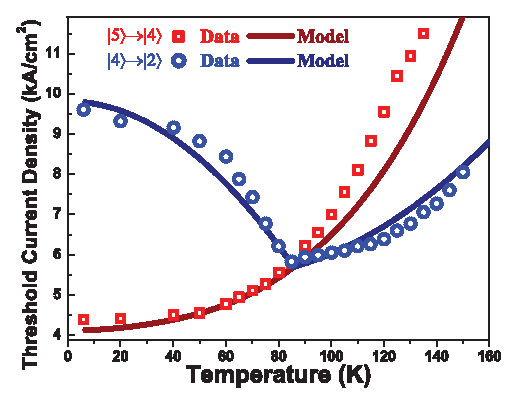
\includegraphics[width=4.25in]{chpt3/chpt3_crossover}
\caption[Model results for transition thresholds]{\textnormal{\textbf{Model results for transition thresholds.}}  Observed and modeled temperature-dependent threshold current densities for the two optical transitions.  Red symbols indicate thresholds for the \trans{5}{4} transition and blue symbols the \trans{4}{2} transition.  A crossover in thresholds is seen near $85~\textnormal{K}$.  Before this crossover, the \trans{4}{2} transition threshold decreases with increasing temperature.  A sharp kink is observed in the \trans{4}{2} threshold when it becomes lower than that of the transition \trans{5}{4}.  These features are reproducible with a conventional QC rate equation model with temperature-dependent parameters, the results of which are indicated by solid lines.}
\label{chpt3:crossover}
\end{figure}

Threshold current densities provide direct means for comparing observed data with the model results.  In using our rate equation model to find threshold current densities, we look for roots of the expression $S_{u\ell}(J)$ as a function of temperature; that is, when $S_{u\ell}(J)=0$, we have a threshold condition.  Figure~\ref{chpt3:crossover} shows a comparison of observed data (open symbols) and calculated thresholds (solid lines).  Using three fitting parameters, our rate equation model is able to provide an excellent reproduction of our observed data.  The three fitting parameters used each control primarily one ``feature'' of the plotted data.  First, by scaling the \trans{5}{4} waveguide loss $\alpha_{w54}$, we match the observed and calculated values of threshold current density for transition \trans{5}{4} over the full temperature range.  Second, by scaling the \trans{4}{2} waveguide loss $\alpha_{w42}$, we match the observed and calculated values of threshold for \trans{4}{2} for $T>85$~K.  This is the temperature range where transition \trans{4}{2} behaves like a conventional QC transition, and where transport through the transition \trans{5}{4} lasing channel is not available since \trans{5}{4} has yet to reach threshold.  Our final fitting parameter is the injection efficiency $\eta_\textit{inj}$ into state \ket{5} and the \emph{k}-space state \ket{4}.  Decreasing $\eta_\textit{inj}$ has the effect of increasing the separation in thresholds for the two transitions for $T<85$~K.

To achieve the fit between observed and calculated data shown in Fig.~\ref{chpt3:crossover}, $\alpha_{w54}$ was scaled by a factor of 4.6, $\alpha_{w42}$ was scaled by a factor of 0.1, and $\eta_\textit{inj}$ was set to 0.88.  The large scaling factor for the transition \trans{5}{4} loss is not surprising, since free carrier loss calculated by the Drude model usually results in an under-estimate \cite{Liu:JQE:2008}.  The extremely small scaling factor for the transition \trans{4}{2} loss needed to reconcile observed and calculated thresholds reflects the effects of \emph{k}-space non-parabolicity described in Section~\ref{chpt3:section_nonparabolicity}.

\begin{table}[tbp]
\captionsetup{width=2.75in}
\centering
\setstretch{1.2}
\caption[Fitting parameters for the \emph{k}-space model]{Fitting parameters used to match the \emph{k}-space rate equation model to observed data.}
\vspace{-0.1in}
\begin{tabular*}{2.75in}{@{\extracolsep{\fill}} c c c }
\toprule
& scaling value & final value\\
\cline{2-3}
$\alpha_{w54}$ & 4.6 & 34~cm\sup{-1}\\
$\alpha_{w42}$ & 0.1 & 0.52~cm\sup{-1}\\
$\eta_\textit{inj}$ & & 0.88\\
\hline
\end{tabular*}
\label{chpt3:tab3}
\end{table}

We were particularly keen on confirming that a \emph{k}-space transition model could reproduce three key features observed in the theshold behavior of the \trans{5}{4} and \trans{4}{2} transitions; those were
\begin{enumerate}
  \setstretch{1.0}
  \setlength{\itemsep}{0pt}
\item the unconventional threshold behavior of the \trans{4}{2} laser transition that decreases then increases with temperature;
\item the crossing of the \trans{5}{4} and \trans{4}{2} laser thresholds; and
\item the sharp kink in the temperature-dependent evolution of the \trans{4}{2} transition threshold at the crossover point.
\end{enumerate}
As clearly seen in Fig.~\ref{chpt3:crossover}, the \emph{k}-space rate equation model is able to accurately reproduce these key features.

A more thorough understanding of the model details may be useful in understanding the origin of the rapid decrease in transition \trans{4}{2} threshold in the 50--85~K temperature range and the sharp kink in the \trans{4}{2} transition at the crossover point.  Since our system of equations represents two coupled optical transitions, each $S_{u\ell}(J)$ has four possible solutions, but real roots for only two.  Each solution represents a different physical state of the system:
\begin{enumerate}
  \setstretch{1.0}
  \setlength{\itemsep}{0pt}
\item a solution for when both transitions are lasing (a real root for both $S_{54}$ and $S_{42}$);
\item a solution for when transition \trans{5}{4} is lasing and transition \trans{4}{2} is not (a real root for only $S_{54}$);
\item a solution for when transition \trans{4}{2} is lasing and transition \trans{5}{4} is not (a real root for only $S_{42}$);
\item a solution for when neither transition is lasing (no real roots).
\end{enumerate}
\begin{figure}[tbp]
\centering
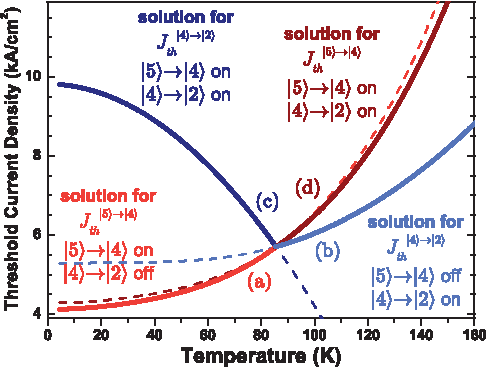
\includegraphics[width=4.25in]{chpt3/chpt3_crossover_model}
\caption[Model results for transition thresholds]{\textnormal{\textbf{Model results for transition thresholds.}}  Modeled temperature-dependent threshold current densities for the two optical transitions.  Four solutions exist for each $S_{u\ell}(T)$; only two are physically meaningful.  The physically meaningful solutions correspond to (i) when a single transition reaches threshold and (ii) when both transitions have reached threshold.  The physically meaningful portions of the solutions are plotted in bold lines.}
\label{chpt3:crossover_model}
\end{figure}
These solutions ``cross'' in temperature when transition \trans{5}{4} and transition \trans{4}{2} have the same threshold.  Furthermore, each solution is only meaningful for a limited set of conditions.  For example, at $T=40$~K, we see four plotted values in Fig.~\ref{chpt3:crossover_model}, two for each optical transition.  Of the two values that correspond to threshold for the \trans{5}{4} transition (red lines \textit{a} and \textit{d}), one value corresponds to when \trans{5}{4} is on and \trans{4}{2} is off, and the other corresponds to when both \trans{5}{4} and \trans{4}{2} are on.  Since the values for the \trans{4}{2} transition (blue lines \emph{b} and \emph{c}) are both larger than the values for the \trans{5}{4} transition, the \trans{5}{4} threshold is less than the \trans{4}{2} threshold.  Thus, the physically meaningful solutions at $T=40$~K are represented by lines \emph{a} and \emph{c}.

With this understanding of the rate equation model, it is now easier to identify the origin of some of the unique threshold behavior features.  While an increased LO phonon transition rate partially contributes to the rapid improvement in the \trans{4}{2} threshold around 55--85~K, the improvement is more aptly recast as a degradation in the \trans{5}{4} threshold, reflecting the fact that, when transition \trans{5}{4} is lasing, the \trans{4}{2} path is carrier-starved.  The kink at the threshold crossover results from a transition between two different operating regimes of the laser: the regime where \trans{5}{4} has a lower threshold and the regime where \trans{4}{2} has a lower threshold.

%To get the simulation to match the data, we used three fitting parameters.  Each parameter is a different knob that controls a different part of the solution.
%
%This, in fact, is what results as the physical ``kink'' in the \trans{4}{2} data at the threshold crossing point.
%
%
%and the apparent rapid change in performance with temperature in the 60--80~K range.
%
%The rapid improvement in the 4?2 threshold around 60--80 K is more aptly recast as a degradation in the 5?4 threshold.
%

\subsection{Cavity-length--dependence of Threshold Crossover}

The extremely low loss associated with the \trans{4}{2} transition results in a marked length-dependence of the two transition thresholds.  As in a typical QC laser, the \trans{5}{4} loss is dominated by waveguide loss for most cavity lengths; mirror loss and waveguide loss are comparable for only very short cavity lengths ($L\leq1$~mm).  In contrast, the \trans{4}{2} \emph{k}-space transition total loss is dominated by mirror loss for even very large cavity lengths.  Thus, since $\alpha_m=-\frac{1}{L}\ln(R)$, thresholds current densities decrease substantially faster with cavity length for transition \trans{4}{2} than they do for transition \trans{5}{4}.  The result is especially noticeable in temperature at which the threshold crossover occurs.  Figure~\ref{chpt3:model_cross_temp} plots calculated threshold crossover vs.\ cavity length, and we can see that, because the net gain increases with increasing cavity length for \trans{4}{2}, the crossover temperature decreases with increasing cavity length.


\begin{figure}[tbp]
\centering
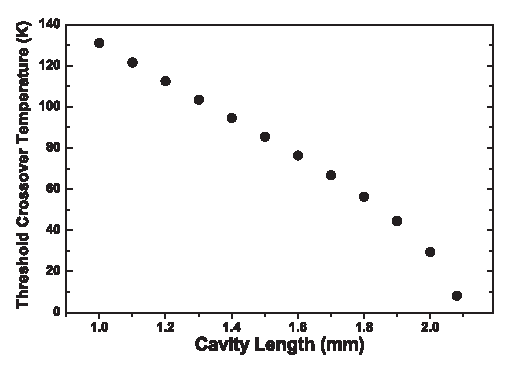
\includegraphics[width=3.8in]{chpt3/chpt3_model_cross_temp}
\caption[Cavity length dependence of transition threshold crossover temperature]{\textnormal{\textbf{Cavity length dependence of transition threshold crossover temperature.}}  Resulting from the extremely low optical loss of the \trans{4}{2} transition, the temperature at which the two transition thresholds cross is highly dependent on cavity length.  Here, the rate equation model results are shown.  Laser data confirm this behavior.}
\label{chpt3:model_cross_temp}
\end{figure}


\section{Conclusions \& Future Directions}
\subsection{Summary}

The work presented in this chapter began with the investigation of a novel QC architecture: the use of an excited state lasing transition.  Because of the extreme flexibility afforded by the general QC concept, unique designs that radically depart from the conventional QC configuration are relatively simple to implement.  However, it is this exact same flexibility to innovate that led us to the primary result of this work so far.  By injecting into an excited state optical transition, other lower-lying transitions also with large oscillator strengths were present in the active region; indeed, we confirmed lasing from such a lower-lying transition.  Because of the unique configuration of our particular laser design, population inversion was not achieved at the $\Gamma$ point in the band structure for the lower transition.  But, because electrons were injected via LO phonon scattering into a high \emph{k}-space position, local population inversion high in \emph{k}-space resulted in high \emph{k}-space laser action.  While both transitions lase simultaneously under certain conditions, the high \emph{k}-space transition is anti-correlated with the primary, excited state laser transition.  A rate equation model based on incorporating a high \emph{k}-space optical transition reproduces the characteristic features of the observed temperature-dependent emission behavior.

To be sure, the demonstration of high \emph{k}-space lasing represents a departure from the conventional approaches to semiconductor lasers.  In semiconductor lasers, because of charge carriers' propensity for extremely fast momentum relaxation \cite{Rudin:PRB:1990} \cite{Alcalde:PRB:1997}, they accumulate at band extrema---\emph{i.e.}, near $k=0$ in direct-gap semiconductors.  Conventional wisdom thus holds that the ``interesting'' device-level physics happens at these band extrema, including population inversion for lasing.  This behavior is universal among diode lasers \cite{Alferov:NobelLecture} \cite{Kroemer:NobelLecture}, interband quantum well lasers \cite{Olafsen:book}, and QC lasers.

The history of QC lasers is decorated with unique methods for obtaining laser action.  Laser transitions with one state being a virtual state have been demonstrated both through Bloch gain \cite{Terazzi:NPhys:2007} \cite{Revin:APL:2008} and stimulated Raman scattering \cite{Troccoli:Nature:2005}.  In every semiconductor injection mechanism to date though, inversion is achieved from electron populations in quasi-equilibrium and thermally distributed around the  $\Gamma$-point.  Our finding of \emph{k}-space injection via LO phonons adds yet another fundamentally unique mechanism to the list of QC-based innovations.

In studying high \emph{k}-space laser transitions, one cannot help but draw a parallel to the hot-hole (p-Ge) laser \cite{Shastin:OQE:1991:p-Ge} \cite{Brunderman:book}.  Here, a combination of large crossed electric and magnetic fields preferentially populates the light hole band of a bulk semiconductor by trapping electrons in cyclotron orbits at high \emph{k}-space, while the applied electric field sweeps holes out of the heavy hole band through streaming motion \cite{Pinson:PR:1964}.  Once these streaming holes in the heavy hole band reach the energy of an optical phonon, a scattering path opens where they can then repopulate the light hole band.  In the work presented here, instead of using externally applied electric and magnetic fields, we employ the optical phonons, a process intrinsic to the material.


\subsection{Future Direction: \emph{Intentionally} created \emph{k}-space lasers}

The possibility of designing intersubband devices that make more cognizant use of full \emph{k}-space population distributions provides a variety of intriguing advantages and possible applications.  The decoupling in energy of the optical emission and reabsorption processes is one point on which high \emph{k}-space transitions are fundamentally superior to $\Gamma$-point transitions.  It is certainly possible that high \emph{k}-space transitions will one day lead to higher performing QC lasers.  But other means may exist to capitalize on the high \emph{k}-space concept.

In addition to the decoupling of emission and absorption, another interesting result of the built-in non-parabolicity is the range over which the transition ``tunes'' as it moves in \emph{k}-space.  If one can make a global population inversion for subbands that are pumped at high \emph{k}-space, an additional method for creating tunable QC lasers could be realized.  Today's most tunable QC sources rely on broadening the gain spectrum by a number of means: rough interfaces \cite{Tsujino:APL:2005:roughness}, bound-to-continuum designs \cite{Wittman:JQE:2008:btc}, diagonal transitions \cite{Yao:JQE:2009}, etc.  Placed in an external cavity setup \cite{Wysocki:APB:2008} or a DFB array \cite{Lee:APL:2007:array}, these methods can yield tunability in the range of 100~cm\sup{-1}.  In comparison, the non-optimized \emph{k}-space transition in our laser had a tuning range in \emph{k}-space of about 16~meV, or 130~cm\sup{-1}.  Coupling a high \emph{k}-space transition with other broadening mechanisms could ultimately yield much better spectral coverage out of a single laser device.

Extension of the \emph{k}-space concept need not be strictly limited to QC lasers.  Our demonstration of the usefulness of electrons in highly non-equilibrium states could be useful in other semiconductor and opto-electronic devices and systems.  For example, in indirect bandgap semiconductors such as silicon, achieving laser action through the traditional across-gap mechanism has proven elusive.  The ability to use non-equilibrium electrons, \emph{e.g.} populating a ``state'' at the $\Gamma$-point, could expose new possible routes to achieving lasing in these systems.

%These additional tools are precious additions to the �intersub-band toolbox� for tackling difficult problems (for example, in achieving intersub-band lasers using a silicon-based heterostructure). In the latter case, the complicated dispersion of the valence band, usually seen as an unwelcome complication, could be used to engineer a population inversion in k-space.
%
%For example, our demonstration of lasing using electrons in a highly non-equilibrium state may have uses in other systems, such as indirect gap semiconductors like Si and Ge.  Achieving laser action through traditional across-gap mechanisms has proven elusive.

%it can be more general than just qc.

Before exploring the strategic use of high \emph{k}-space transitions, one must confront and resolve a primary challenge: how best to populate the high \emph{k}-space state?  We have demonstrated that the momentum transfer associated with LO phonons can accomplish the task; Yamanishi \emph{et al.} have demonstrated a similar upper laser state population mechanism \cite{Yamanishi:OptExp:2008}.  However, using the electron-LO phonon process may ultimately prove to be a transport bottleneck that limits performance \cite{Yao:JQE:2009}.  Another possibility might be taking advantage of the (normally) parasitic satellite \emph{k}-space valleys.  Given sufficient electron energy above the band edge, electron-electron scattering between valleys is extremely rapid.  Innovation on this front will be necessary to realize a practical high \emph{k}-space device.


\subsection{Future Direction: Further develop the excited state concept}

The work on QC lasers specifically designed to maximize the large oscillator strengths accompanying excited state transitions is ongoing. Whether this design strategy will ultimately be useful for long-wavelength lasing remains to be proven.  As demonstrated throughout the chapter, achieving high performance at long-wavelengths is hindered by multiple challenges.  While the excited state strategy addresses some of these challenges by compensating for large optical losses with larger oscillator strengths, the strategy itself introduces some new challenges.  For example, excited state transitions can make achieving population inversion even more difficult.  When more lower states are added below the optical transition, as in excited state structures, the ratio $\left(1-\frac{\tau_\ell}{\tau_{u\ell}}\right)$ becomes smaller.  A carefully balanced design will ultimately yield the best trade-off between this effect of decreased lifetimes and maximizing oscillator strength.

Another primary challenge for the excited state strategy that must be overcome is the huge energy drop between optical transitions, the effective $\Delta_\textit{inj}$.  While such a large $\Delta_\textit{inj}$ can aggravate the problem of resonant absorption in the injector region, it also leads to a significant reduction in wall-plug efficiency.  Careful design can minimize injector region resonant absorption.  A potential fix for the hit to wall-plug efficiency might be engineering two optical transitions of the same energy in the active region.  By creating a ``double photon'' structure, energy that would normally be surrendered to the lattice can be used to create more photons.


%Certainly, QC designs that sufficiently suppress thermal emission out of the upper laser state will be required, which in the excited state design presented in this chapter severely limited the thermal performance.


\subsection{Future Direction: Correlated photons}

In this chapter, we have shown that simultaneous lasing is in principle possible from stacked transitions.  In the QC design and devices presented here, the lower optical transition did not achieve population inversion at the $\Gamma$ point due to a lack of states into which electrons could scatter.  However, more careful design that specifically seeks to empty out the lowest active region state could create an active region with stacked transitions that both attain population inversion at the $\Gamma$ point.  In this case, simultaneous lasing could lead to the generation of correlated photons.

One primary challenge of generating correlated photons by this strategy will be to maximize the transport path where electrons make two successive $\Gamma$-point optical transitions.  Another transport path, where electrons scatter to the middle state of the stacked transitions via LO phonons, should be minimized.  %This favored setup, however, could in fact be a natural state of the system, since non-parabolicity will lead to different lasing energies for the lower transition of the two transport paths.


%and minimize the number of electrons that scatter via LO phonons into the middle state, and then make an optical transition only from the lower transition.  Yet, with the added k-space dynamics and non-parabolicity, this could work itself out on its own.




%
%\bibliographystyle{kale3}
%\bibliography{biblio}
%\end{document} 